%% bare_jrnl.tex
%% V1.3
%% 2007/01/11
%% by Michael Shell
%% see http://www.michaelshell.org/
%% for current contact information.
%%
%% This is a skeleton file demonstrating the use of IEEEtran.cls
%% (requires IEEEtran.cls version 1.7 or later) with an IEEE journal paper.
%%
%% Support sites:
%% http://www.michaelshell.org/tex/ieeetran/
%% http://www.ctan.org/tex-archive/macros/latex/contrib/IEEEtran/
%% and
%% http://www.ieee.org/



% *** Authors should verify (and, if needed, correct) their LaTeX system  ***
% *** with the testflow diagnostic prior to trusting their LaTeX platform ***
% *** with production work. IEEE's font choices can trigger bugs that do  ***
% *** not appear when using other class files.                            ***
% The testflow support page is at:
% http://www.michaelshell.org/tex/testflow/


%%*************************************************************************
%% Legal Notice:
%% This code is offered as-is without any warranty either expressed or
%% implied; without even the implied warranty of MERCHANTABILITY or
%% FITNESS FOR A PARTICULAR PURPOSE! 
%% User assumes all risk.
%% In no event shall IEEE or any contributor to this code be liable for
%% any damages or losses, including, but not limited to, incidental,
%% consequential, or any other damages, resulting from the use or misuse
%% of any information contained here.
%%
%% All comments are the opinions of their respective authors and are not
%% necessarily endorsed by the IEEE.
%%
%% This work is distributed under the LaTeX Project Public License (LPPL)
%% ( http://www.latex-project.org/ ) version 1.3, and may be freely used,
%% distributed and modified. A copy of the LPPL, version 1.3, is included
%% in the base LaTeX documentation of all distributions of LaTeX released
%% 2003/12/01 or later.
%% Retain all contribution notices and credits.
%% ** Modified files should be clearly indicated as such, including  **
%% ** renaming them and changing author support contact information. **
%%
%% File list of work: IEEEtran.cls, IEEEtran_HOWTO.pdf, bare_adv.tex,
%%                    bare_conf.tex, bare_jrnl.tex, bare_jrnl_compsoc.tex
%%*************************************************************************

% Note that the a4paper option is mainly intended so that authors in
% countries using A4 can easily print to A4 and see how their papers will
% look in print - the typesetting of the document will not typically be
% affected with changes in paper size (but the bottom and side margins will).
% Use the testflow package mentioned above to verify correct handling of
% both paper sizes by the user's LaTeX system.
%
% Also note that the "draftcls" or "draftclsnofoot", not "draft", option
% should be used if it is desired that the figures are to be displayed in
% draft mode.
%
\documentclass[journal,twocolumn]{IEEEtran}
%
% If IEEEtran.cls has not been installed into the LaTeX system files,
% manually specify the path to it like:
% \documentclass[journal]{../sty/IEEEtran}


% Some very useful LaTeX packages include:
% (uncomment the ones you want to load)


% *** MISC UTILITY PACKAGES ***
%
%\usepackage{ifpdf}
% Heiko Oberdiek's ifpdf.sty is very useful if you need conditional
% compilation based on whether the output is pdf or dvi.
% usage:
% \ifpdf
%   % pdf code
% \else
%   % dvi code
% \fi
% The latest version of ifpdf.sty can be obtained from:
% http://www.ctan.org/tex-archive/macros/latex/contrib/oberdiek/
% Also, note that IEEEtran.cls V1.7 and later provides a builtin
% \ifCLASSINFOpdf conditional that works the same way.
% When switching from latex to pdflatex and vice-versa, the compiler may
% have to be run twice to clear warning/error messages.






% *** CITATION PACKAGES ***
%
%\usepackage{cite}
% cite.sty was written by Donald Arseneau
% V1.6 and later of IEEEtran pre-defines the format of the cite.sty package
% \cite{} output to follow that of IEEE. Loading the cite package will
% result in citation numbers being automatically sorted and properly
% "compressed/ranged". e.g., [1], [9], [2], [7], [5], [6] without using
% cite.sty will become [1], [2], [5]--[7], [9] using cite.sty. cite.sty's
% \cite will automatically add leading space, if needed. Use cite.sty's
% noadjust option (cite.sty V3.8 and later) if you want to turn this off.
% cite.sty is already installed on most LaTeX systems. Be sure and use
% version 4.0 (2003-05-27) and later if using hyperref.sty. cite.sty does
% not currently provide for hyperlinked citations.
% The latest version can be obtained at:
% http://www.ctan.org/tex-archive/macros/latex/contrib/cite/
% The documentation is contained in the cite.sty file itself.






% *** GRAPHICS RELATED PACKAGES ***
%
\ifCLASSINFOpdf
  % \usepackage[pdftex]{graphicx}
  % declare the path(s) where your graphic files are
  % \graphicspath{{../pdf/}{../jpeg/}}
  % and their extensions so you won't have to specify these with
  % every instance of \includegraphics
  % \DeclareGraphicsExtensions{.pdf,.jpeg,.png}
\else
  % or other class option (dvipsone, dvipdf, if not using dvips). graphicx
  % will default to the driver specified in the system graphics.cfg if no
  % driver is specified.
  % \usepackage[dvips]{graphicx}
  % declare the path(s) where your graphic files are
  % \graphicspath{{../eps/}}
  % and their extensions so you won't have to specify these with
  % every instance of \includegraphics
  % \DeclareGraphicsExtensions{.eps}
\fi
% graphicx was written by David Carlisle and Sebastian Rahtz. It is
% required if you want graphics, photos, etc. graphicx.sty is already
% installed on most LaTeX systems. The latest version and documentation can
% be obtained at: 
% http://www.ctan.org/tex-archive/macros/latex/required/graphics/
% Another good source of documentation is "Using Imported Graphics in
% LaTeX2e" by Keith Reckdahl which can be found as epslatex.ps or
% epslatex.pdf at: http://www.ctan.org/tex-archive/info/
%
% latex, and pdflatex in dvi mode, support graphics in encapsulated
% postscript (.eps) format. pdflatex in pdf mode supports graphics
% in .pdf, .jpeg, .png and .mps (metapost) formats. Users should ensure
% that all non-photo figures use a vector format (.eps, .pdf, .mps) and
% not a bitmapped formats (.jpeg, .png). IEEE frowns on bitmapped formats
% which can result in "jaggedy"/blurry rendering of lines and letters as
% well as large increases in file sizes.
%
% You can find documentation about the pdfTeX application at:
% http://www.tug.org/applications/pdftex





% *** MATH PACKAGES ***
%
%\usepackage[cmex10]{amsmath}
% A popular package from the American Mathematical Society that provides
% many useful and powerful commands for dealing with mathematics. If using
% it, be sure to load this package with the cmex10 option to ensure that
% only type 1 fonts will utilized at all point sizes. Without this option,
% it is possible that some math symbols, particularly those within
% footnotes, will be rendered in bitmap form which will result in a
% document that can not be IEEE Xplore compliant!
%
% Also, note that the amsmath package sets \interdisplaylinepenalty to 10000
% thus preventing page breaks from occurring within multiline equations. Use:
%\interdisplaylinepenalty=2500
% after loading amsmath to restore such page breaks as IEEEtran.cls normally
% does. amsmath.sty is already installed on most LaTeX systems. The latest
% version and documentation can be obtained at:
% http://www.ctan.org/tex-archive/macros/latex/required/amslatex/math/





% *** SPECIALIZED LIST PACKAGES ***
%
%\usepackage{algorithmic}
% algorithmic.sty was written by Peter Williams and Rogerio Brito.
% This package provides an algorithmic environment fo describing algorithms.
% You can use the algorithmic environment in-text or within a figure
% environment to provide for a floating algorithm. Do NOT use the algorithm
% floating environment provided by algorithm.sty (by the same authors) or
% algorithm2e.sty (by Christophe Fiorio) as IEEE does not use dedicated
% algorithm float types and packages that provide these will not provide
% correct IEEE style captions. The latest version and documentation of
% algorithmic.sty can be obtained at:
% http://www.ctan.org/tex-archive/macros/latex/contrib/algorithms/
% There is also a support site at:
% http://algorithms.berlios.de/index.html
% Also of interest may be the (relatively newer and more customizable)
% algorithmicx.sty package by Szasz Janos:
% http://www.ctan.org/tex-archive/macros/latex/contrib/algorithmicx/




% *** ALIGNMENT PACKAGES ***
%
%\usepackage{array}
% Frank Mittelbach's and David Carlisle's array.sty patches and improves
% the standard LaTeX2e array and tabular environments to provide better
% appearance and additional user controls. As the default LaTeX2e table
% generation code is lacking to the point of almost being broken with
% respect to the quality of the end results, all users are strongly
% advised to use an enhanced (at the very least that provided by array.sty)
% set of table tools. array.sty is already installed on most systems. The
% latest version and documentation can be obtained at:
% http://www.ctan.org/tex-archive/macros/latex/required/tools/


%\usepackage{mdwmath}
%\usepackage{mdwtab}
% Also highly recommended is Mark Wooding's extremely powerful MDW tools,
% especially mdwmath.sty and mdwtab.sty which are used to format equations
% and tables, respectively. The MDWtools set is already installed on most
% LaTeX systems. The lastest version and documentation is available at:
% http://www.ctan.org/tex-archive/macros/latex/contrib/mdwtools/


% IEEEtran contains the IEEEeqnarray family of commands that can be used to
% generate multiline equations as well as matrices, tables, etc., of high
% quality.


%\usepackage{eqparbox}
% Also of notable interest is Scott Pakin's eqparbox package for creating
% (automatically sized) equal width boxes - aka "natural width parboxes".
% Available at:
% http://www.ctan.org/tex-archive/macros/latex/contrib/eqparbox/





% *** SUBFIGURE PACKAGES ***
%\usepackage[tight,footnotesize]{subfigure}
% subfigure.sty was written by Steven Douglas Cochran. This package makes it
% easy to put subfigures in your figures. e.g., "Figure 1a and 1b". For IEEE
% work, it is a good idea to load it with the tight package option to reduce
% the amount of white space around the subfigures. subfigure.sty is already
% installed on most LaTeX systems. The latest version and documentation can
% be obtained at:
% http://www.ctan.org/tex-archive/obsolete/macros/latex/contrib/subfigure/
% subfigure.sty has been superceeded by subfig.sty.



%\usepackage[caption=false]{caption}
%\usepackage[font=footnotesize]{subfig}
% subfig.sty, also written by Steven Douglas Cochran, is the modern
% replacement for subfigure.sty. However, subfig.sty requires and
% automatically loads Axel Sommerfeldt's caption.sty which will override
% IEEEtran.cls handling of captions and this will result in nonIEEE style
% figure/table captions. To prevent this problem, be sure and preload
% caption.sty with its "caption=false" package option. This is will preserve
% IEEEtran.cls handing of captions. Version 1.3 (2005/06/28) and later 
% (recommended due to many improvements over 1.2) of subfig.sty supports
% the caption=false option directly:
%\usepackage[caption=false,font=footnotesize]{subfig}
%
% The latest version and documentation can be obtained at:
% http://www.ctan.org/tex-archive/macros/latex/contrib/subfig/
% The latest version and documentation of caption.sty can be obtained at:
% http://www.ctan.org/tex-archive/macros/latex/contrib/caption/




% *** FLOAT PACKAGES ***
%
%\usepackage{fixltx2e}
% fixltx2e, the successor to the earlier fix2col.sty, was written by
% Frank Mittelbach and David Carlisle. This package corrects a few problems
% in the LaTeX2e kernel, the most notable of which is that in current
% LaTeX2e releases, the ordering of single and double column floats is not
% guaranteed to be preserved. Thus, an unpatched LaTeX2e can allow a
% single column figure to be placed prior to an earlier double column
% figure. The latest version and documentation can be found at:
% http://www.ctan.org/tex-archive/macros/latex/base/



%\usepackage{stfloats}
% stfloats.sty was written by Sigitas Tolusis. This package gives LaTeX2e
% the ability to do double column floats at the bottom of the page as well
% as the top. (e.g., "\begin{figure*}[!b]" is not normally possible in
% LaTeX2e). It also provides a command:
%\fnbelowfloat
% to enable the placement of footnotes below bottom floats (the standard
% LaTeX2e kernel puts them above bottom floats). This is an invasive package
% which rewrites many portions of the LaTeX2e float routines. It may not work
% with other packages that modify the LaTeX2e float routines. The latest
% version and documentation can be obtained at:
% http://www.ctan.org/tex-archive/macros/latex/contrib/sttools/
% Documentation is contained in the stfloats.sty comments as well as in the
% presfull.pdf file. Do not use the stfloats baselinefloat ability as IEEE
% does not allow \baselineskip to stretch. Authors submitting work to the
% IEEE should note that IEEE rarely uses double column equations and
% that authors should try to avoid such use. Do not be tempted to use the
% cuted.sty or midfloat.sty packages (also by Sigitas Tolusis) as IEEE does
% not format its papers in such ways.


%\ifCLASSOPTIONcaptionsoff
%  \usepackage[nomarkers]{endfloat}
% \let\MYoriglatexcaption\caption
% \renewcommand{\caption}[2][\relax]{\MYoriglatexcaption[#2]{#2}}
%\fi
% endfloat.sty was written by James Darrell McCauley and Jeff Goldberg.
% This package may be useful when used in conjunction with IEEEtran.cls'
% captionsoff option. Some IEEE journals/societies require that submissions
% have lists of figures/tables at the end of the paper and that
% figures/tables without any captions are placed on a page by themselves at
% the end of the document. If needed, the draftcls IEEEtran class option or
% \CLASSINPUTbaselinestretch interface can be used to increase the line
% spacing as well. Be sure and use the nomarkers option of endfloat to
% prevent endfloat from "marking" where the figures would have been placed
% in the text. The two hack lines of code above are a slight modification of
% that suggested by in the endfloat docs (section 8.3.1) to ensure that
% the full captions always appear in the list of figures/tables - even if
% the user used the short optional argument of \caption[]{}.
% IEEE papers do not typically make use of \caption[]'s optional argument,
% so this should not be an issue. A similar trick can be used to disable
% captions of packages such as subfig.sty that lack options to turn off
% the subcaptions:
% For subfig.sty:
% \let\MYorigsubfloat\subfloat
% \renewcommand{\subfloat}[2][\relax]{\MYorigsubfloat[]{#2}}
% For subfigure.sty:
% \let\MYorigsubfigure\subfigure
% \renewcommand{\subfigure}[2][\relax]{\MYorigsubfigure[]{#2}}
% However, the above trick will not work if both optional arguments of
% the \subfloat/subfig command are used. Furthermore, there needs to be a
% description of each subfigure *somewhere* and endfloat does not add
% subfigure captions to its list of figures. Thus, the best approach is to
% avoid the use of subfigure captions (many IEEE journals avoid them anyway)
% and instead reference/explain all the subfigures within the main caption.
% The latest version of endfloat.sty and its documentation can obtained at:
% http://www.ctan.org/tex-archive/macros/latex/contrib/endfloat/
%
% The IEEEtran \ifCLASSOPTIONcaptionsoff conditional can also be used
% later in the document, say, to conditionally put the References on a 
% page by themselves.





% *** PDF, URL AND HYPERLINK PACKAGES ***
%
%\usepackage{url}
% url.sty was written by Donald Arseneau. It provides better support for
% handling and breaking URLs. url.sty is already installed on most LaTeX
% systems. The latest version can be obtained at:
% http://www.ctan.org/tex-archive/macros/latex/contrib/misc/
% Read the url.sty source comments for usage information. Basically,
% \url{my_url_here}.





% *** Do not adjust lengths that control margins, column widths, etc. ***
% *** Do not use packages that alter fonts (such as pslatex).         ***
% There should be no need to do such things with IEEEtran.cls V1.6 and later.
% (Unless specifically asked to do so by the journal or conference you plan
% to submit to, of course. )


% correct bad hyphenation here
\hyphenation{op-tical net-works semi-conduc-tor}

%% load necessary packages
% \documentclass[paper=a4, fontsize=10pt,headings=small]{scrartcl}
% \documentclass[paper=a4, fontsize=10pt,headings=small]{scrartcl}
% \documentclass[journal,onecolumn]{IEEEtran}
% \documentclass[paper=a4, fontsize=10pt,parskip=half,headings=small]{scrartcl}
\usepackage{check-short}
\usepackage{overpic}
\usepackage{multirow}
\usepackage{enumerate}


%% set author information etc
\title{Limitations of traditional models for perfusion}
\author{Constantin Sandmann, Erik A. Hanson, Alexander Malyshev,  Arvid Lundervold, Jan Modersitzki, Erlend Hodneland }
\date{\today}


%% define some local commands
\newcommand{\Qso}{Q_{\mathrm{so}}}
\newcommand{\Qsi}{Q_{\mathrm{si}}}
\newcommand{\ca}{c_\mathrm{a}}
\newcommand{\CBV}{\mathrm{CBV}}
\newcommand{\MTT}{\mathrm{MTT}}
\newcommand{\cout}{c_{\mathrm{v}}}
\newcommand{\Pa}{P_{\mathrm{a}}}
\newcommand{\Pout}{P_{\mathrm{v}}}
\newcommand{\Perf}{P}
\newcommand{\Perfv}{P_{\mathrm{v}}}
\newcommand{\Perfs}{P_{\mathrm{s}}}
\newcommand{\Flow}{F}
\newcommand{\vq}{\mathbf{q}}
\newcommand{\vx}{\mathbf{x}}
\newcommand{\vy}{\mathbf{y}}
\newcommand{\vdx}{\mathbf{dx}}



%define SI-units, since we want to be able to easily change them
% \newcommand{\simu}{k\pascal$\cdot$\second} %CH: I have problems compiling with the cdot
\newcommand{\simu}{k\pascal\second}
\newcommand{\siFmm}{\milli\meter\cubed\per\second}
\newcommand{\siFml}{\milli\litre\per\second}
\newcommand{\siQmm}{\milli\meter\cubed\per\second\per\milli\meter\cubed}
\newcommand{\siPml}{\milli\litre\per\minute\per100\milli\litre}
\newcommand{\siq}{\milli\meter\cubed\per\second\per\milli\meter\squared}
\newcommand{\siml}{\milli\litre}
\newcommand{\siphimm}{\milli\meter\cubed\per\milli\meter\cubed}
\newcommand{\siJ}{\milli\mol\per\second\per\milli\meter\squared}
\newcommand{\siphi}{\milli\meter\cubed\per\milli\meter\cubed}
\newcommand{\sirho}{\milli\gram\per\milli\meter\cubed}
\newcommand{\siQtilde}{\milli\gram\per\second\per\milli\meter\cubed}
\newcommand{\sic}{\milli\mol\per\milli\meter\cubed}
\newcommand{\simm}{\milli\meter\cubed}

%\newcommand{\siP}{\cubic\milli\meter\per\second\per\cubic\milli\meter}
%\newcommand{\siP}{\milli\meter\cubed\per\second}
%\newcommand{\siPml}{\milli\litre\per\second}
%\newcommand{\siQtilde}{\milli\gram\per\second\per\milli\meter\cubed}
%\newcommand{\siQ}{\milli\meter\cubed\per\second\per\milli\meter\cubed}
%\newcommand{\sirho}{\milli\gram\per\milli\meter\cubed}
%\newcommand{\sic}{\milli\mol\per\milli\meter\cubed}
%\newcommand{\siPn}{\milli\litre\per\minute\per100\milli\litre}
%\newcommand{\simm}{\milli\meter\cubed}


%define misc commands
\newcommand{\missingsource}{\textcolor{red}{[?]}}
\newlength{\fwd}
\newlength{\fht}

%--------------------------------------------------------------------------------------------
%--------------------------------------------------------------------------------------------
% Here begins the document, remove "draft" option in document class to include images
%--------------------------------------------------------------------------------------------
%--------------------------------------------------------------------------------------------

\begin{document}
	%--------------------------------------------------
	% Title Page=
	%--------------------------------------------------
	\maketitle
%	\tableofcontents

	%ABSTRACT MODIFIED TO FOCUS ON THE ANALYSIS AND NOT THE NUERICAL EXPERIMENTS OR THE POROUS MEDIA FLOW.
	\begin{abstract}
		\textbf{Objective:}
		In perfusion imaging the usage of traditional one-compartment models to estimate haemodynamic parameters like perfusion, blood volume and mean transit times is widespread. In this paper we set up a mathematical framework, clearly revealing limitations of traditional models related to perfusion recovery.
		\textbf{Methods:}
		Theoretical details for the transitional understanding of perfusion are derived for the case then image resolution goes beyond the spatial scale of the capillary tissue. 
		To achieve this, a continuous flow model for propagation of a tracer for such tissue was developed, and the signal intensity map was used for perfusion estimation by traditional models.
		\textbf{Results:}
		Traditional one-compartment models are equivalent to the continuous flow model if upstream effects can be accounted for.
		It is demonstrated that traditional models are accurately recovering perfusion when applied to the entire domain but are not meaningful when applied to smaller portions of the system, resulting in overestimation of perfusion.
		Evidence of real patient data is provided, indicating that this effect might also be observed in real-life applications.
		\textbf{Conclusion:}
		We find that traditional models for perfusion overestimate blood flow when applied to only parts of a coupled system. Estimation of the blood volume is stable and can also be applied in coupled systems.
		\textbf{Significance:}
		%Results indicate that clinical perfusion results will be accurate, as long as the control volume consists of capillary tissue and has direct arterial and venous connection.
		Awareness should be draw to uncertainties in voxel wise perfusion estimates when coupled flow is expected. For future perfusion studies the development of continuous and coupled PDE models are highly recommended.
	\end{abstract}

	%--------------------------------------------------
	%--------------------------------------------------
	% Section: Introduction
	%--------------------------------------------------
	%--------------------------------------------------
	\section{Introduction}

	Quantitative measurements of hemodynamic medical parameters based on tracer kinetic modeling are widespread both in research and in clinical practice \cite{sourbron13,Feng2013,Chen2011}. 
	In the present work, we focus on mathematical models to estimate blood perfusion (cerebral blood flow, CBF), blood volume (cerebral blood volume, CBV), and mean transit time (MTT) of the brain from dynamic image data using intravascular tracers. 

	While hardware limitations in medical imaging for decades have confined studies to only handle larger tissue regions or full organs, modern imaging technology and voxel based analysis give rise to aspirations about detailed perfusion maps with sub-millimeter precision. Examples of estimated parameter maps can be found in \cite{Feng2013,Chen2011}. We expect the development to continue and that imaging systems will reach a resolution where a single capillary system spans over several voxels. Capillary tissue is here understood as tissue perfused by capillaries.
	Quantitative perfusion maps, as well as other parameter maps arising from tracer kinetic modeling, can be combined with anatomical information and have proven to be of particular value in e.g. stroke studies or localization of trauma.
	Among the physiological parameters obtainable from tracer kinetic modeling, CBF has been found particularly difficult to describe reliably on a voxel-basis \cite{kudo10}.
	These limitations are caused by issues of the numerical implementation \cite{kudo10}, but might also depend on over-simplified dynamic models, which were originally designed to describe larger volumes of interest \cite{zierler00}.	

	Most commonly, perfusion can be understood as the delivery of arterial blood to the capillary system.
	There have been several approaches to clarify this concept in a continuous sense.
	In \cite{calamante03}, dispersion of the arterial input function was simulated using Navier-Stokes equations.
	It was shown that neglecting to account for dispersion can have adverse impact on perfusion measurements.
	In \cite{Henkelman1990}, the problem of scale dependent continuous perfusion was discussed. Perfusion defined as flow entering a voxel will scale with voxel size, 
	%  as volume flow (perfusion) scales differently than surface flow (flux). 
	and this notion of perfusion is therefore inappropriate.	
	More recently a two-compartment model was introduced as a precise definition of local perfusion \cite{sourbron14}.	
	However, evaluation of the proposed modeling is still pending.

	% THE TWO FOLLOWING PARAGAPHS ARE SWOPED 

	In this work we focus on the validity of traditional perfusion models.
	We  demonstrate that traditional models like deconvolution or the maximum slope model are able to recover the perfusion accurately if applied to the entire domain fed by the incoming flow.
	However, when applying the traditional models to isolated parts of the full system, we find that local perfusion in coupled systems is not straightforward to define.
	In order to highlight this issue, two theoretical definitions of voxel-wise perfusion are presented: A definition $\Perfv$ describing the local inflow into a voxel, but otherwise not fulfilling the traditional ideas of perfusion, and then a tailored definition of perfusion $\Perfs$ for continuous models.

The concepts are illustrated by simulations of flow in a tissue patch with one inlet, one outlet, and a capillary system in between.
	A directional flow field for the patch is set up according to Darcy's law from porous media flow \cite{Darcy56}.
	Contrast agent propagation in this patch is simulated using transport equations.
	We show that a discretized version of the continous flow system can be equivalently described by a coupled set of multiple traditional one-compartment models, in line with the physical environment where each control volume is feeding its direct neighbors.

	
	Our results show that traditional models tend to overestimate $\Perfs$ and underestimate $\Perfv$ if they are applied only to parts of the full system.
	Analytic results are given, which show how the recovered perfusion depends on all upstream flow and not only on the local value.
	We also show results indicating that overestimation of perfusion due to coupling might also be present in real data.

	
	%--------------------------------------------------
	%--------------------------------------------------
	% Section: Traditional models
	%--------------------------------------------------
	%--------------------------------------------------

	%THIS SECTION IS NOT CHANGED
	\section{Traditional Models for perfusion} \label{sec:traditional}

	In this section we describe the convolution- and the maximum slope model, two widely used one-compartment pharmacokinetic models for measurements of CBF and CBV \cite{Feng2013,Chen2011,kudo10}.
	For the remaining, they are referred to as \emph{traditional} models.

	Let $\Omega_i$ be an arbitrary control volume with one inlet and one outlet, and let $C(t)$ denote the average contrast agent (CA) concentration within $\Omega_i$ at timepoint $t$.
	The traditional models assume that the change of concentration at timepoint $t$ can be described by the ordinary differential equation 
	\begin{equation}\label{eq:classicgeneral}
		C'(t) = \Pa\ca(t) - \Pout\cout(t), \quad C(0) = 0.
	\end{equation}
	Here, $\ca,\cout$ are the plasma CA concentrations at the inlet and outlet of $\Omega_i$ and $\Pa,\Pout$ is the flow at these locations.
	In the following, it is assumed that the plasma tracer concentration $\ca$ at the inlet is known.
	In clinical practice this can be accounted for by measuring $\ca$ in a feeding artery \cite{ostergaard96}.
	Since $\cout$ is usually unknown, additional assumptions need to be made if one wants to reconstruct $\Pa$ from a given tissue curve $C$. The convolution model and the maximum slope (MS) model diverge in further assumptions.

	

	%----------------------------------------------------------
	% Subsection: The Convolution Model: Theory and Implementation
	%----------------------------------------------------------	
	\subsection{The Convolution Model}\label{sec:conv}
	For the deconvolution model, one approach is to assume there is an unknown probability distribution of transit times $h$ through $\Omega_i$, cf. \cite{sourbron13}. 
	This leads to
	\begin{equation}
		\Pout\cout(t) = \Pa(h\ast\ca)(t) := \Pa\int_0^t \ca(s) h(t-s) \diffint s.
	\end{equation}
	Combining this with \eqref{eq:classicgeneral} yields $C'(t) = \Pa\ca(t)-\Pa (h\ast\ca)(t)$.
	Integrating this equation and using basic properties of the convolution one obtains the general solution
	\begin{equation}
		C(t) = (I\ast\ca)(t).
		\label{eq:conv}
	\end{equation}
	where the \emph{impulse response function} $I$ is defined as $I(t) := \Pa(1-\int_0^t h(s) \diffint s)$.
	The task of identifying $I(t)$ given a tissue curve $C(t)$ and an arterial input function $\ca(t)$ is a deconvolution problem.
	If $I(t)$ is recovered, $\Pa$ can subsequently be estimated as $\Pa = \max_{t} I(t)$.
	There are several methods to perform the deconvolution.
	A standard approach using Fourier-based algorithms is sensitive to the presence of noise \cite{ostergaard96}.
	Another class of deconvolution algorithms gaining increasing attention are based on Bayesian modeling \cite{boutelier12}.
	However the numerical handling is still difficult since complex and error-prone numerical integration has to be performed \cite{boutelier12}.
	A popular class among deconvolution algorithms is based on singular value decomposition (SVD) \cite{ostergaard96}.
	These algorithms have shown to be robust for a reasonable noise level.
	Also, they can be easily adapted to be robust against delays in tracer arrival using block-circular structures (bSVD cf. \cite{wu03}).
	In order to identify the impulse response function $I(t)$ from applied data, we hence decided to use the bSVD model as proposed in \cite{wu03}.

	
	
	%----------------------------------------------------------
	% Subsection: The Maximum Slope Model
	%----------------------------------------------------------
	\subsection{The Maximum Slope Model}\label{sec:ms}	
	In the MS model it is assumed that when $\ca$ has its maximum, only a negligible amount of CA is leaving the system \cite{klotz99}.
	For this time interval, \eqref{eq:classicgeneral} reduces to 
	\begin{equation}
		C'(t) = \Pa\ca(t), \quad C(0) = 0.
	\end{equation}
	One can see that if $\ca$ has a maximum, also $C'$ must have a maximum since stationarity in $\Pa$ is assumed.
	Hence, it holds that
	\begin{equation}\label{eq:MS}
		\Pa = \frac{\max_{t}C'(t)}{\max_{t}\ca(t)}.
	\end{equation}

	
	
	%--------------------------------------------------
	%--------------------------------------------------
	% Section: The synthetic model
	%--------------------------------------------------
	%--------------------------------------------------	
	\section{A Synthetic Model for Capillary Flow}\label{sec:synthetic}

	The validity of the traditional methods relies on a control volume with only one inlet and one outlet, and that the control volumes are not feeding each other.
	These assumptions may easily be violated when we locally describe CA propagation through a larger volume.
	For this type of model system we instead expect a set of coupled equations where each voxel can be regarded as an inlet for surrounding voxels.

	Hence, in order to make a realistic synthetic model for capillary flow, we decided to describe the CA propagation as a spatially coupled transport process, i.e. using partial differential equations (PDE) for transport. This PDE model is used for validation of the traditional models. 

	
	A major difference between our coupled flow model and traditional tracer kinetic modeling is the normalization of the flow field.
% In traditional models normalization is performed with respect to the volume and leads to the units of perfusion [\si{\siQmm}], cf. \cite{sourbron13}.
	To avoid a discretization dependent flow field for the PDE model, we instead of perfusion use vector valued surface fluid flux $\vq = \vq(\vx)$ with units [\si{\siq}] as the fluid carrying quantity, in agreement with geoscience and porous media simulation theory.
	The fluid flux is a vector field describing the volume of fluid per unit time flowing across a sliced unit area of the sample.
	A detailed outline of how the flow field was obtained can be found in Section~\ref{sec:flow}.
	%Apart from the normalization with respect to surface, the assumptions of stationarity in the fluid flux are in agreement with standard pharmacokinetic modelling \cite{sourbron13}.



			
	%--------------------------------------------------
	% Subsection: Modeling the Contrast Agent Transport
	%--------------------------------------------------	

	%HERE I CHANGED THE ORDER OF THE SECTIONS. THE TRANSPORT IS DESCRIBED FIRST 		ACCOMPANIED BY CORRESPONDING ANALYSIS.
	\subsection{A Model for Indicator Dilution}\label{sec:transport}

	%The introduced framework in Section \ref{sec:flow} does not relate flow to propagation of a contrast agent. 
	This section describes a model for  CA propagation in the tissue as it is homogeneously dissolved in the evolving fluid.
	We assume that the CA is entering the domain along with the fluid flowing into the ROI via the source, and similarly extracted at a sink.
	%The resulting CA concentration map is a simulation of the CA concentrations observed within real MRI measurements.

	In order to define meaningful and continuous contrast agent concentrations, we first describe CA concentration in an (arbitrarily) small tissue volume $\Omega_\varepsilon$.
	% where $C_i(t):= C(x_i,t)$ and $\phi_i := \phi(x_i)$ are assumed to be constant within $\Omega_i$.
	Let $V_\varepsilon$ be the volume of $\Omega_\varepsilon$ and let $v_\varepsilon$ be the blood volume within the same control region.
	Letting the control region go towards zero volume, the porosity $\phi(\vx) :=  \lim_{\varepsilon \to 0} v_\varepsilon/V_\varepsilon$ reflects the local, relative volume of the vascular system. The simplification of porosity as a continuous function is frequently performed in flow simulations.
	The flux $\vq(\vx)$ [\si{\siq}] as well as the porosity $\phi(\vx)$ [\si{\siphi}] are assumed to be stationary and hence independent of time.	
	We further introduce $C = C(\vx,t)$ and $c = c(\vx,t)$ as the average CA concentration within $V_\varepsilon$ and $v_\varepsilon$, respectively.
	By definition, we obtain the relation $C(\vx,t) = \phi(\vx)  c(\vx,t)$.
	The rate of change of tracer molecules within a control volume $\Omega_i$ can hence be phrased as
	\begin{equation}
		\frac{d}{dt} \int_{\Omega_i}C  \diffint \vx = \int_{\Omega_i}	\frac{d}{dt} (\phi c) \diffint \vx = \int_{\Omega_i} \phi \frac{d c}{dt} \diffint \vx,
		\label{eq:dmdt}
	\end{equation}	
	where the assumption of stationary $\phi(\vx)$ was used.
	Assuming mainly transport and marginal diffusion, the change in tracer mass within $\Omega_i$ occurs from advective flow and the source and sink field $Q(\vx)$.
	Let us write the source- and the sink term as $Q(\vx) = \Qsi(\vx) + \Qso(\vx)$ where $\Qsi(\vx) < 0$ is the sink and $\Qso(\vx) > 0$ is the source, and zero elsewhere. 
	Note that $\int_\Omega Q  \vdx = 0$. 
	% The change in contrast agent at time point $t$ from fluid entering the control volume can be written as
	% \begin{equation}
	% 	-\int_{ \partial \Omega_i}c(\vq \cdot n)\diffint s + \int_{\Omega_i}\ca Q_{so} \diffint x + \int_{\Omega_i}cQ_{si} \diffint x,
	% 	\label{eq:surfflux}
	% \end{equation}
	% where $n(x)$ is the outward unit normal on $\partial \Omega_i$.
	% In standard pharmacokinetic modeling, $\ca = \ca(x,t)$ is referred to as the arterial input function (AIF).
	Using \eqref{eq:dmdt} and following the principle of conservation of tracer molecules, we model the contrast agent concentration in a control volume $\Omega_i$ as
	\begin{align}
		& \int_{\Omega_i} \phi \frac{d c}{dt} \diffint \vx + \int_{ \partial \Omega_i}c(\vq \cdot \mathbf{n}) \diffint \mathbf{A}
		 = \int_{\Omega_i}(\ca Q_{so} \diffint \vx + c Q_{si}) \diffint \vx.
		\label{eq:conteq}
	\end{align}
	where $\mathbf{n}(\vx)$ is the outward unit normal on $\partial \Omega_i$.
% 	Now, let the contrast agent concentrations, porosity, volume fluxes, and surface flux be continuous functions of space and time. 
	Equation (\ref{eq:conteq}) is consistent with the continuity equation on local form
	\begin{equation}
		\left\vert
		\begin{alignedat}{2}
			\phi \frac{\partial c}{\partial t} + \nabla \cdot (c\vq) &= \ca\Qso + c\Qsi \qquad	&\vx &\in \Omega, \ t>0,  \\
			c(\vx,t) &= 0 																			 	&\vx &\in \Omega, \ t=0.
		\end{alignedat}
		\right\vert
		\label{eq:conteqlocal}
	\end{equation}
	where we also added the initial condition $c(\vx,0) = 0$ in line with the physical problem of no tracer at $t = 0$.
	Equation \eqref{eq:conteqlocal} is a linear transport equation in $c(\vx,t)$. 
	Following \cite{evans98}, \eqref{eq:conteqlocal} admits a unique local solution.


	%--------------------------------------------------
	% Subsection: Relating New Model with Old Model
	%--------------------------------------------------
\subsection{Relating the transport equation model with the traditional deconvolution model for perfusion}\label{sec:NewAndOld}
	In this section we describe how the continuous model is related to the traditional deconvolution model.
	We will show that in the continuous model the flow into each voxel can be described as a traditional model with arterial input determined by adjacent upstream voxels.

	Let us start by modeling the CA concentration in a given voxel $\Omega_i$ using traditional models.
	For sake of simplicity we assume that $Q_{\mathrm{so}} = Q_{\mathrm{si}} = 0$ within that voxel.
	Note that it is possible to extend the following approach also to voxels where this is not the case.
	Define the outward normal vector $n$ and areas (voxel faces) of inflow and outflow over the boundary as $S_{\mathrm{in}} := \{ \vx \in \partial \Omega_i: \ \vq \cdot \mathbf{n} < 0 \}$ and $S_{\mathrm{out}}:= \{ \vx \in \partial \Omega_i: \ \vq \cdot \mathbf{n} > 0 \}$ respectively.
	For the domain $\Omega_i$ we define the arterial input $c_{\mathrm{in}}$ as the weighted average of the tracer flux across $S_{\mathrm{in}}$
	\begin{equation}\label{eq:cin}
	 	c_{\mathrm{in}}(t):= \frac{\int_{S_{\mathrm{in}}}c \cdot (\vq \cdot \mathbf{n}) \diffint \mathbf{A}}{\int_{S_{\mathrm{in}}} \vq \cdot \mathbf{n} \diffint \mathbf{A}}.
	\end{equation}
	We define perfusion $\Perfv$ within $\Omega_i$ in line with the definition as the total feeding fluid inflow divided by the volume,
	\begin{equation}\label{eq:perflocal}
		\Perfv :=-\frac{1}{\mathrm{Vol}( \Omega_i)}\int_{S_{\mathrm{in}}} \vq \cdot \mathbf{n} \diffint \mathbf{A}.
	\end{equation}
	Given an incompressible flow, let us now assume that the rate of fluid entering the region is the same as the rate of fluid leaving it. 
	Further, let $c_i(t)$ denote the average CA concentration within $\Omega_i$.
	%Further assume that the tracer concentration is constant within a voxel $\Omega_i$, leading to the notation $c(x,t) = c_i(t) ~\forall ~ x \in \Omega_i$.
	Then it holds that $\Perfv=P_{\mathrm{out}}$ and we can describe $c_i$ by the traditional model \eqref{eq:classicgeneral},
	\begin{equation}\label{eq:singlevoxel}
		(\phi c_i)'(t)  = \Perfv (c_\mathrm{in}(t)  - c_\mathrm{out}(t)).
	\end{equation}
	% COMPLETE CALCULATION:
	% \begin{align}
	% 	(\phi_ic_i)'(t)  &= \frac{1}{\Vol(\Omega_i)}\left(\sum_{j=0}^k p_j c_j(t) - \left(\sum_{j=0}^k p_j\right) c_i(t)\right)\\
	% 	 				 &= \sum_{j=0}^k P_j c_{j}(t) - P c_i(t)\\
	% 	         &= P(\tfrac{1}{P}\sum_{j=0}^k P_j c_{j}(t) - c_i(t))\\
	% 			 &= P(c_{\mathrm{in}}(t) - c_i(t))\\
	% \end{align}
	% Here $p_j$ is absolute flow, $P_j:=p_j/\Vol(\Omega_i)$ the corresponding normalized perfusion for arterial input $j$ and $P:=\sum_{j=0}^k P_j$ the total perfusion for the voxel.
	% Solving the above ODE leads to
	% \[
	% 	C_i(t) = \phi_i (J_i\ast c_{\mathrm{in}})(t), \text{ for }J_i(t) = \tfrac{P}{\phi_i}\exp(-(P/\phi_i)t).
	% \]	
	Note that the upwind-discretization described in Section~\ref{sec:transport} models each voxel as a well-mixed compartment: it is assumed that the CA concentration at the outflow $S_\mathrm{out}$ equals the concentration within the voxel and that the concentration at the inflow is the concentration within the adjacent voxels.

	%I PROPOSE TO SHORTEN THE REST OF THIS SECTION. BY NOW I BELEVE THE READER IS CONFORTABLE WITH THE FACT THAT LOCAL FLOW IS DEPENDENT ON UPSTREAM VOXELS.

	In this case it follows that \eqref{eq:singlevoxel} reduces to $(\phi c_i)'(t) = \Perfv (c_\mathrm{in}(t) - c_i(t))$ 
	with solution
	\begin{equation}\label{eq:voxelcurve}
		C_i(t) = \phi_i(J_i*c_{\mathrm{in}})(t)
			\text{ for } J_i(t)=(\Perfv/\phi_i)e^{- (\Perfv/\phi_i)t}.
	\end{equation}
	The arterial input $c_{\mathrm{in}}$ is determined by \eqref{eq:cin}, which recursively depends on all upstream voxels until the global arterial input is reached.
	To verify this relationship numerically, we simulated a tissue curve $C_i(t)$ using both the continuous PDE model as well as analytical recursive convolution by \eqref{eq:voxelcurve}.
	We refer to the latter approach as \textit{local convolution}. The two curves have an almost perfect match, as seen in Figure~\ref{fig:VoxelComp} (left).	

	As a direct consequence, it follows by recursion that the concentration at a voxel $i$ can be written as a convolution of the (global) arterial input function with a weighted average of all upstream impulse response functions.
	Deconvolving a tissue concentration $C_i$ with the global AIF will yield an impulse response function which depends not only on the local flow and porosity, but on flow and porosity of all upstream voxels.
	% In the special case that transport is occurring only along one row of voxels, as e.g. in the top row of our synthetic example, the concentration in voxel $i$ is given by
	% \begin{equation}
	% 	C_i(t) = \phi_i (J_1\ast \dots \ast J_{i-1})\ast\ca)(t).
	% 	\label{eq:C_recur}
	% \end{equation}
	% where $J_i(s):=p_i\mathrm{exp}(- p_i(s))$ for $p_i=\Perfv^i/\phi_i$.
	% An analytic expression for the convolution of finitely many functions $J_i$ can be found in \cite{Kordecki97}.
	% Following , the convolution of exponential functions with pairwise different parameters $p_i$ is given by
	% \begin{equation}\label{eq:C_recur}
	% 	(J_1\ast \dots \ast J_n)(s) = \sum_{i=1}^n \frac{\Pi_{j=1}^n p_j}{\Pi_{j=1,j\neq i}^n(p_j-p_i)}e^{-p_is}.
	% \end{equation}
	% See \cite{Kordecki97} for the case $p_i=p_j$ for some $i,j$.
	This relationship was also confirmed experimentally: Figure~\ref{fig:VoxelComp} (right) shows the impulse response function determined by analytical recursive convolution and the numerically achieved impulse response function obtained from deconvolving a tissue curve of the continuous model with the global arterial input function. 
	The simulation was performed at location (1,20) of the software phantom.
	The two curves coincide almost perfectly, highlighting the validity of the established theory.

These results show that the PDE model and the convolution model are equal in terms of local, voxelwise flow estimates if the convolution model is applied with the local arterial input. 
Also, the impulse response function obtained by convolution of the global arterial input function is identical to an analytical recursive convolution along all upstream voxels. 
This clearly demonstrates that the perfusion which is recovered by traditional models will depend on all upstream flow.
However, for meaningful interpretation of the perfusion the entire streamline length within the capillary system needs to be taken into consideration, where the blood is providing the tissue with nutrients and oxygen. 
%These results also support the idea presented in the next section that pointwise perfusion can be regarded a globally constant quantity along the streamlines, as it can only be estimated when the entire streamline characteristics are known.
	\fwd = .4\textwidth
	\fht = .1\textheight	
	\begin{figure*}
		{
		\small
		% \begin{tabular}{p{\fwd} p{\fwd}}
		\begin{tabular}{c c}
			% This file was created by matlab2tikz.
%
%The latest updates can be retrieved from
%  http://www.mathworks.com/matlabcentral/fileexchange/22022-matlab2tikz-matlab2tikz
%where you can also make suggestions and rate matlab2tikz.
%
\definecolor{mycolor1}{rgb}{0.00000,0.44700,0.74100}%
\definecolor{mycolor2}{rgb}{0.85000,0.32500,0.09800}%
%
\begin{tikzpicture}

\begin{axis}[%
width=0.951\fwd,
height=0.75\fht,
at={(0\fwd,0\fwd)},
scale only axis,
xmin=0,
xmax=40,
xlabel={time [s]},
ymin=0,
ymax=2.5e-07,
ylabel={$C$ $\text{[mmol/mm}^\text{3}\text{]}$},
axis background/.style={fill=white},
legend style={legend cell align=left,align=left,draw=white!15!black}
]
\addplot [color=mycolor1,solid,very thick]
  table[row sep=crcr]{%
0	0\\
0.4	0\\
0.8	0\\
1.2	0\\
1.6	0\\
2	5.62373487759478e-11\\
2.4	1.09810271021085e-09\\
2.8	6.76053034703798e-09\\
3.2	2.13478347753626e-08\\
3.6	4.56056649657982e-08\\
4	7.67693039618778e-08\\
4.4	1.10760368816952e-07\\
4.8	1.43746597983364e-07\\
5.2	1.72821999990385e-07\\
5.6	1.96160012105964e-07\\
6	2.12907090713985e-07\\
6.4	2.22973323725445e-07\\
6.8	2.26804741960865e-07\\
7.2	2.25178885025859e-07\\
7.6	2.19040032343215e-07\\
8	2.09376955393214e-07\\
8.4	1.97139176006753e-07\\
8.8	1.83184972235038e-07\\
9.2	1.6825381701405e-07\\
9.6	1.5295649926078e-07\\
10	1.3777726549853e-07\\
10.4	1.23083485704354e-07\\
10.8	1.09139475580703e-07\\
11.2	9.61220627108628e-08\\
11.6	8.41362598740187e-08\\
12	7.32300105168483e-08\\
12.4	6.34074188236187e-08\\
12.8	5.46401838538925e-08\\
13.2	4.68771886140848e-08\\
13.6	4.00523095626387e-08\\
14	3.4090617904463e-08\\
14.4	2.89131601344388e-08\\
14.8	2.44405364930844e-08\\
15.2	2.05954798314946e-08\\
15.6	1.73046252038486e-08\\
16	1.44996421001143e-08\\
16.4	1.21178699857602e-08\\
16.8	1.01025854633713e-08\\
17.2	8.40299542178553e-09\\
17.6	6.97404198461131e-09\\
18	5.77607935091924e-09\\
18.4	4.77447355834304e-09\\
18.8	3.93916172160292e-09\\
19.2	3.24419737926786e-09\\
19.6	2.66730266166506e-09\\
20	2.18943870651418e-09\\
20.4	1.79440465920876e-09\\
20.8	1.46846847064005e-09\\
21.2	1.20003289411346e-09\\
21.6	9.79336326007395e-10\\
22	7.98187748378252e-10\\
22.4	6.49733970754416e-10\\
22.8	5.28256526672998e-10\\
23.2	4.28995952016572e-10\\
23.6	3.48000282397405e-10\\
24	2.81995444125054e-10\\
24.4	2.28274651883307e-10\\
24.8	1.84604584011355e-10\\
25.2	1.49146036254608e-10\\
25.6	1.20387064957272e-10\\
26	9.70868785116934e-11\\
26.4	7.82288318545415e-11\\
26.8	6.29812300119354e-11\\
27.2	5.06646643040334e-11\\
27.6	4.07249116439323e-11\\
28	3.27104678363883e-11\\
28.4	2.62539803586422e-11\\
28.8	2.10569311946487e-11\\
29.2	1.68770204325555e-11\\
29.6	1.35178038053597e-11\\
30	1.0820183236205e-11\\
30.4	8.65544366249652e-12\\
30.8	6.91955310729552e-12\\
31.2	5.5285112362483e-12\\
31.6	4.41455486319452e-12\\
32	3.52306811834916e-12\\
32.4	2.81007005409287e-12\\
32.8	2.2401727856489e-12\\
33.2	1.78492607969931e-12\\
33.6	1.42147458549083e-12\\
34	1.13147177733343e-12\\
34.4	0\\
34.8	0\\
35.2	0\\
35.6	0\\
36	0\\
36.4	0\\
36.8	0\\
37.2	0\\
37.6	0\\
38	0\\
38.4	0\\
38.8	0\\
39.2	0\\
39.6	0\\
};
\addlegendentry{Convolution};

\addplot [color=mycolor2,dashed,very thick]
  table[row sep=crcr]{%
0	0\\
0.4	0\\
0.8	0\\
1.2	0\\
1.6	0\\
2	5.3279568073074e-11\\
2.4	1.07821521955639e-09\\
2.8	6.71290754043026e-09\\
3.2	2.12564956013061e-08\\
3.6	4.54228810841506e-08\\
4	7.64315332182225e-08\\
4.4	1.10213523840219e-07\\
4.8	1.42958770768866e-07\\
5.2	1.71785826132747e-07\\
5.6	1.94889508729946e-07\\
6	2.11432221500284e-07\\
6.4	2.21334146149828e-07\\
6.8	2.25046160287466e-07\\
7.2	2.23346407714781e-07\\
7.6	2.17176667633836e-07\\
8	2.07521150089304e-07\\
8.4	1.95323644243314e-07\\
8.8	1.81436224500391e-07\\
9.2	1.66592199968555e-07\\
9.6	1.51396589797636e-07\\
10	1.3632847936435e-07\\
10.4	1.21750799207446e-07\\
10.8	1.07924182119412e-07\\
11.2	9.50225094085739e-08\\
11.6	8.31485298722586e-08\\
12	7.2348531031234e-08\\
12.4	6.26254832899861e-08\\
12.8	5.39503908539349e-08\\
13.2	4.62717953679953e-08\\
13.6	3.95235135517039e-08\\
14	3.36307690244454e-08\\
14.4	2.85149175130422e-08\\
14.8	2.40969765219252e-08\\
15.2	2.03001649700339e-08\\
15.6	1.70516423039829e-08\\
16	1.4283615166056e-08\\
16.4	1.19339562230449e-08\\
16.8	9.94645645486966e-09\\
17.2	8.27081040255549e-09\\
17.6	6.86241431416851e-09\\
18	5.68204011719055e-09\\
18.4	4.6954337247387e-09\\
18.8	3.87287421966553e-09\\
19.2	3.18872072804604e-09\\
19.6	2.62096602035629e-09\\
20	2.15080978220791e-09\\
20.4	1.76225980427895e-09\\
20.8	1.44176580276721e-09\\
21.2	1.17788797530892e-09\\
21.6	9.61000531233148e-10\\
22	7.83029147436785e-10\\
22.4	6.37220457950388e-10\\
22.8	5.1794117711445e-10\\
23.2	4.20504195487211e-10\\
23.6	3.41018904827157e-10\\
24	2.76263049750932e-10\\
24.4	2.23573527582697e-10\\
24.8	1.80753733306562e-10\\
25.2	1.45995250370183e-10\\
25.6	1.17811903729239e-10\\
26	9.4984407302507e-11\\
26.4	7.65140460587736e-11\\
26.8	6.15840282729948e-11\\
27.2	4.95273231768238e-11\\
27.6	3.97999619242864e-11\\
28	3.19589252105288e-11\\
28.4	2.56438694661132e-11\\
28.8	2.05620562202835e-11\\
29.2	1.64759471844691e-11\\
29.6	1.31930121953556e-11\\
30	1.05573697632337e-11\\
30.4	8.44294196192858e-12\\
30.8	6.74785807138353e-12\\
31.2	5.38988595036491e-12\\
31.6	4.30270767561291e-12\\
32	3.43288752398976e-12\\
32.4	2.73740677349094e-12\\
32.8	2.18166182862043e-12\\
33.2	1.73784050750156e-12\\
33.6	1.38360654329319e-12\\
34	1.10103495034139e-12\\
34.4	0\\
34.8	0\\
35.2	0\\
35.6	0\\
36	0\\
36.4	0\\
36.8	0\\
37.2	0\\
37.6	0\\
38	0\\
38.4	0\\
38.8	0\\
39.2	0\\
39.6	0\\
};
\addlegendentry{PDE};

\end{axis}
\end{tikzpicture}% & \input{./figs/IDecVSIAna.tikz}\\
		\end{tabular}
		}
		\caption{Left: Red curve shows the tissue concentrations ($C$) of the continuous PDE model at location [32,35]. Blue curve shows recursive convolution by \eqref{eq:voxelcurve} with experimental value of $\Perfv=\SI{5328}{\siPml}$ at the given location and $c_{\mathrm{in}}$ taken locally from upstream voxels around the simulated voxel. The two curves have an almost perfect overlap. Note that the numbers used for the perfusion is unrealisticely high since normalization is performed with respect to the volume of only one voxel. Right: Red curve shows the computed impulse response functions (IR) at location [1,20] using the global arterial input function. Blue curve shows the analytic impulse response function given by a convolution over all upstream flow. The two curves have an almost perfect overlap. These numerical experiments support that the computed impulse response function by traditional methods is not the directly feeding impulse response function, but rather a recursive impulse response function depending on all upstream voxels.}\label{fig:VoxelComp}
	\end{figure*}


	%--------------------------------------------------
	% Subsection: Converting Flow to Perfusion
	%--------------------------------------------------

	%THIS SECTION HAS BEEN CHANGED TO FOCUS MORE TOWARD COUPLED CAPILLARY SYSTEMS. I KNOW THAT THIS APPROACH CAN BE DICUSSED, BUT I FEEL THERE ARE TWO LINES OF ARGUMENTATION HERE: 
	%ONE APROAVH IS THE ONE OF SOURBRON. HE ARGUES THAT WHEN BLOOD FLOWS FROM A VOEL TO ANOTHER WE DONT HAVE ANY INFORMATION ABOUTH THE FRATION OF BLOOD BEING ARTERIAL AND THE AMOUNT THAT HAS BEEN PERFUSED UPSTREAM AND CURRENTLY IS VENAL BLOOD. HIS 'FIELD' MODEL ACCOUNTS FOR THIS (BUT IS NOT A 1C MODEL). 
	%THE OTHER APPROACH IS THE FLOW IN COUPLED CAPILARY SYSTEMS APROACH. HERE WE ASSUME THAT THE PERFUSION IS TAKING PLACE ACROSS VOXELS. IE. WE HAVE A MILIMETER VOXEL SCALE WHERE THE STREMLINES GO THROUGH THE CAPILARY SYSTEMS. IN THIS SETTING THE RELATION BETWEEN FLOW/FLUX AND PERFUSION CAN BE CONSIDERED IN THE 1C-FRAMEWORK WE ARE USING. 

	\subsection{Relating Flow with Perfusion}\label{sec:flux2perf}
	The flow model described in \eqref{eq:flowmodel} uniquely determines the flux field $\vq(\vx)$. 
	However, in pharmacokinetic modeling the parameter of interest is usually CBF, which we will denote by $\Perf (\vx)$ as the voxelwise field of perfusion. Surface flux and perfusion are physically distinct, and there are at least two differences between $\vq(\vx)$ and $\Perf (\vx)$. 
	First, flux is a vector field and perfusion is a scalar field. Second, the flux is normalized to a surface area and the perfusion is normalized to a volume. 
	Hence the flux describes flow and transport over a surface separating spatial regions, while the perfusion describes blood leaving/entering a compartment within a given volume. 	
	%In the following we describe a method for converting flux into perfusion, motivated by our need to compare the PDE based ground-truth, vector valued flux field to the scalar valued perfusion field obtained by traditional methods.
More specifically, the common understanding of perfusion
	 
	 $\Perf (\vx)$ is the amount of blood feeding a tissue volume per unit time, with units [\si{\siQmm}]. 
	 In this work we address the  fine scale setting, where the perfusion is taking place on voxel level. At this level, a clearer understanding of how perfusion relates to the flux is desirable.  

	One straightforward approach for converting flux into perfusion could be to estimate the perfusion as the total inflow (or outflow) of fluid (e.g. arterial blood) into a control region per unit time, and then normalizing with the control region volume. 
	This is a valid approach only if the control regions are not feeding each other, and is therefore well-founded for the entire organ,
	in line with the theoretical foundation of traditional compartment models for perfusion where a control region has its own source of feeding arterial blood, independent of neighbour regions. 

	On the other hand, if the control region is a single voxel or a sub-division of a capillary system with sequentially feeding arterial blood, the traditional model assumptions are violated since every control region will feed its neighbours, thus becoming a coupled system of flow. 
	Simply summing the total inflow into a voxel and dividing by the voxel volume will strongly over-estimate the perfusion as the normalization refers to the wrong volume. 
	This phenomenon is demonstrated in Figure~\ref{fig:perfusion-problem} where the volume on the left has the true perfusion of $\Perf_{1} = \Flow_0 /(2V)$ for an incoming flow $\Flow_0$ [$\si{\siFmm}$] and distribution volume $2V$ [$\si{\simm}$]. 
	However, for another discretization as shown in the middle, the perfusion within each of these sub-volumes becomes $\Perf_{2} = F_0/V = 2\Perf_{1}$. 
	Taking the average across the two sub-volumes, it is clear that the perfusion is over-estimated with a factor of two. 
	A discretization dependent perfusion estimate is not recommendable, and the perfusion estimate of $\Perf_{2}$ is clearly wrong. 
	This problematic issue was previously identified by \cite{Henkelman1990}, stating that an incorrect normalization will lead to multiple counting of the same flow, and hence an over-estimation of perfusion.

	\begin{figure}
	    \centering
	    \begin{overpic}[scale=0.3]{figs/perfusion-problem.eps}
	    	\put(10,70){\color{black}$F_0$}
			\put(48,70){\color{black}$F_0$}
			\put(84,70){\color{black}$\Delta F_0$}
			\put(10,33){\color{black}$2V$}
			\put(49,20){\color{black}$V$}
			\put(49,45){\color{black}$V$}
			\put(91,42){\color{black}$\Delta V$}
		\end{overpic}
	    \caption{Perfusion within a small volume. Left: A compartment with volume $2V$ is exposed to a flow $\Flow_0$ [$\si{\siFmm}$] of fluid. By definition, the perfusion within this compartment becomes $\Perf_{1} = \Flow_0/(2V)$. Middle: The same volume is divided into two compartments (e.g. voxels), and the perfusion for each of the compartments becomes $\Perf_{2} = \Flow_0/V = 2\Perf_{1}$. The discrepancy between the two discretizations occurs because the flow is counted twice as it is fed from one voxel to the other. Right: As a solution to the described problem we rather pick out a true distribution volume $\Delta V$ (area in this 2D sketch), which is a small area around a given streamline along the centre line of the grey area. This is the true distribution volume (area in this 2D sketch) which is fed with arterial blood from the incoming fractional flow $\Delta \Flow_0$. The correct perfusion within $\Delta V$ is therefore $\Delta F_0/\Delta V$. The entire compartment can further be divided into similar infinitesimal distribution volumes, thus providing locally correct perfusion estimates.}
	    \label{fig:perfusion-problem}
	\end{figure}

	In the following we introduce a meaningful notion of perfusion for the fine scale continuous model.
	To do this, we will consider distribution volumes which are following the streamlines, as shown in Fig. \ref{fig:perfusion-problem} (right). 	
	For each point of a streamline we will select a small perpendicular disk with radius chosen in such a way that the total flow over each disk is constant along the streamline.

	More precisely, let us consider an arbitrary streamline $S \subseteq \Omega \subseteq \R^3$ of length $l>0$ and parametrization $s:[0,l] \to S$.
	We start by calculating the total flow over a small 2-D disc perpendicular to the streamline.
	Let $\vy \in S$ be an arbitrary location along the streamline. 
	The total flow $F$ over a 2-D disc $B(\vy,R(\vy))$ perpendicular to the flow field $\vq(\vy)$, centered at $\vy$ and with radius $R:S\to\R^+$, is given by
	\begin{equation}
		F(\vy,R(\vy)) = \int_{B(\vy,R(\vy))} \vq(\vx) \cdot \mathbf{n} \diffint \vx \text{ where }\mathbf{n} := \vq(\vy)/\vert \vq(\vy) \vert.
		\label{eq:Fdisc}
	\end{equation}
	In order to calculate the perfusion, we need to establish the volume of a small tube around the streamline.
	We will not consider a tube with constant radius, but one with spatially varying radii $r:[0,l] \to \R^+$.
	The total volume of such a tube is given by
	\begin{equation}
		V(r) = \int_0^l r(u)^2 \pi \diffint u.
	\end{equation}
        Note that $R(\vy):=r(u)$ for some $u \in [0,l]$
        % satisfying $\vy=s(u)$. 
        We define the perfusion at the arbitrary point $\vy$ on the streamline as
	\begin{equation}
		\Perfs(\vy):=  \lim_{\varepsilon \to 0} \frac{F(\vy,\varepsilon R(\vy))}{V(\varepsilon r)} \text{ for } R(\vy):=1/\sqrt{\vert \vq(\vy) \vert}.
		\label{eq:perfusiondef}
	\end{equation}
	%Note that $F(y,\varepsilon r(u))=F(y,\varepsilon R(y))$, and can be interchanged independent of parameterization. 
	In this expression the radii $R(\vy)$ are chosen in such a way that in the limit when $\varepsilon \to 0$, the perfusion is constant along the streamline. 
	To see this, let us assume that $\vq$ is differentiable with Jacobian $J$.
	Using a Taylor expansion of $\vq(\vx)$ around $\vy$, the Lagrange remainder theorem, as well as a change of coordinates $\mathbf{z} = (\vx-\vy)/(\varepsilon R)$ yields 
	 % \begin{align*}
	 % 	F(y,\varepsilon R(y))&=\int_{B(y,\varepsilon R(y))} \nu^\top q(x) \diffint x \\
	 % 	&= \int_{B(y,\varepsilon R(y))} \nu^\top q(y)  + \nu^\top J(\xi) (x-y) \diffint x \\
	 % 	&= \varepsilon^2 \pi  + \int_{B(0,1)} \nu^\top J(\zeta) z(\varepsilon R(y))^3 \diffint z \\
	 % 	&= \varepsilon^2 \left(\pi + \varepsilon \int_{B(0,1)} \nu^\top J(\zeta)z R(y)^3 \diffint z\right)
	 % \end{align*}
	\begin{equation}
		F(\vy,\varepsilon R(\vy))
		= \varepsilon^2 \Big(\pi + \varepsilon \int_{B(0,1)} \mathbf{n}^\top J(\zeta)zR(\vy)^3 \diffint \mathbf{z} \Big)
	\end{equation}
	where $\zeta_i \in (0,z_i)$ for every vector element $i$, and simplifications are due to $R(\vy) = 1/\sqrt{\vert \vq(\vy)} \vert$ and $\mathbf{n}:=\vq(\vy)/\vert \vq(\vy) \vert$.
	Combining this result with \eqref{eq:perfusiondef} yields
	\begin{equation}\label{eq:flux2perf}
		\Perfs(\vy) = \left(\int_0^l r(u)^2 \diffint u\right)^{-1}.
	\end{equation}
	Note that Equation \eqref{eq:flux2perf} is independent of the spatial location $y$ along the streamline, and is an explicit formula for converting flux into perfusion, showing that the perfusion scales with the streamline length $l$, as well as with the geometry of the domain, represented by the radii $r(u)$.


	%--------------------------------------------------
	% Subsection: Estimate the Porosity
	%--------------------------------------------------	
	\subsection{A Method to Estimate Local Porosity}\label{sec:CBV}

	Porosity and CBV have the same definition, and we can therefore state that $\phi \equiv \mathrm{CBV}$. It is known from literature on traditional models \cite{sourbron13} for perfusion that CBV for the entire compartment can be expressed as
	\begin{equation}
		\phi = \frac{\int_0^\infty C(s) \diffint s}{\int_0^\infty \ca(s) \diffint s}.
		\label{eq:CBV}
	\end{equation}
	% where $C(t)$ is the tracer concentration with respect to a well mixed compartment and $\ca(t)$ is the plasma concentration of the arterial input.
	It is not obvious that \eqref{eq:CBV} is valid also for a one-compartment field model where the voxels are feeding each other. 
	We will now show that this is indeed the case.
	
	Let us switch to a discrete setting.
	Consistent with the considerations in Section~\ref{sec:NewAndOld} let us assume that the CA concentration in any voxel can be described by $C_i(t) = \phi_i(J_i\ast c_{\mathrm{in},i})(t)$, where the local arterial input is given by
		$c_{\mathrm{in},i}(t) =1/p(p_0 \ca(t) + \sum_{j \in J} p_jc_j(t))$.
	In this discrete version of \eqref{eq:cin}, $J$ is the set of all adjacent, upstream voxels and $p=p_0 + \sum_{j\in J} p_j$, where $p_0>0$ if voxel $i$ lies within the source field.
	Furthermore let us assume that $\vq$ is a uni-directional flow field and that there is no flow between voxels in the same layer.
		We now use induction to show that $\int_0^\infty c_i(s) \diffint s = \int_0^\infty \ca(s) \diffint s$, then \eqref{eq:CBV} follows.
		Let $I_k$ denote the set of voxels which have $k$ layers of upstream voxels.
		E.g. $I_0$ is the set of all voxels, which have no upstream voxels, $I_1$ is the set of voxels which are fed by $I_0$ and so on.
		Induction will be carried out over $k$.\\
		\textbf{Induction basis:}
		Let $k=0$ and let $i \in I_0$ be arbitrary.
		Since the area under the convolution of two functions equals the product of the area of its factors, $\int_0^\infty c_i(s) \diffint s = \int_0^\infty \ca(s) \diffint s$ and the claim follows.\\
		\textbf{Induction step:}
		Consistent with our assumptions, for any voxel at location $i \in I_{k+1}$ which has the voxels $J \subseteq I_{k}$ as their upstream neighbors, we find the following expression:
		\begin{equation}
			\int_0^\infty c_i(s) \diffint s = \tfrac{1}{P}\int_0^\infty \Big(J_i\ast \big( p_0 \ca(s) + {\textstyle\sum\limits_{j \in J}}p_j c_j(s) \big)\Big)(s) \diffint s
		\end{equation}
		Now \eqref{eq:CBV} follows from straight-forward calculations.
	


	%% LONG VERSION OF THE DISCRETE PROOF
	% 	Let us switch to a discrete setting let the following assumptions hold (see Section~\ref{sec:NewAndOld} for details):
	% 	\begin{enumerate}[({A}1)]
	% 		\item The concentration in any voxel can be written as
	% 	\begin{equation}
	% 		\int_0^\infty c_i(s) \diffint s = \int_0^\infty (J_i\ast c_{\mathrm{in},i})(s) \diffint s.
	% 	\end{equation}
	% 	where $J_i,c_{\mathrm{in},i}:[0,\infty)\to \R$ will be specified in (A2).
	% 	\item In (A1) $J_i:[0,\infty)\to\R$ fulfills $\int_0^\infty J_i(s)\diffint s = 1$ (straight forward calculation) and the local arterial input $c_{\mathrm{in},i}(t)$ is a weighted average of adjacent, upstream voxels $c_j(t)$, where $J$ is the set of adjcacent, upstream voxels and $\ca(t)$, if the voxel lies in the source field:
	% 	\begin{equation}
	% 		c_{\mathrm{in},i}(t) = \tfrac{1}{P}\Big(p_0 \ca(t) + {\textstyle\sum\limits_{j \in J}} p_jc_j(t)\Big),
	% 	\end{equation}
	% 	where $p=p_0 + \sum_{j\in J} p_j$ and $p_0>0$ if voxel $i$ lies within the source field.
	% 	Consistent with \eqref{eq:cin} $p_j$ is absolute flow.
	% 	\end{enumerate}
	%
	% 	\begin{lemma}
	% 		Assume (A1),(A2), a uni-directional flow over voxel faces and that there is no flow between voxels in the same layer.
	% 		Then $\int_0^\infty C_i(s) \diffint s = \phi_i \int_0^\infty \ca(s) \diffint s$ for all voxels.
	% 	\end{lemma}
	% 	\begin{proof}
	% 		We use induction to show that $\int_0^\infty c_i(s) \diffint s = \int_0^\infty \ca(s) \diffint s$, then the claim follows.
	% 		Let $I_k$ denote the set of voxels which have $k$ layers of upstream voxels.
	% 		E.g. $I_0$ is the set of all voxels, which have no upstream voxels, $I_1$ is the set of voxels which are fed by $I_0$ and so on.
	% 		Induction will be carried out over $k$.\\
	% 		\textbf{Induction Basis:}\\
	% 		Let $k=0$ and let $i \in I_0$ be arbitrary. Following (A1) and (A2) it holds that $c_i(t) = (J_i\ast \ca)(t)$.
	% 		Since the area under the convolution of two functions equals the product of the area of its factors, $\int_0^\infty c_i(s) \diffint s = \int_0^\infty \ca(s) \diffint s$ and the claim follows.\\
	% 		\textbf{Induction Assumption:} The claim holds for arbitrary $k \in \N$.\\
	% 		\textbf{Induction Step:}\\
	% 		For any voxel at location $i \in I_{k+1}$ which has the voxels $J \subseteq I_{k}$ as their upstream neighbors, we find the following expression:
	% 		\begin{align*}
	% 			\int_0^\infty c_i(s) \diffint s &\stackrel{\mathclap{\text{(A1)}}}{=} \int_0^\infty (J_i\ast c_{\mathrm{in},i})(s) \diffint s\\
	% 			&= \int_0^\infty c_{\mathrm{in},i}(s)\diffint s \\
	% 			&\stackrel{\mathclap{\text{(A2)}}}{=}  \tfrac{1}{P}\int_0^\infty \Big( p_0 \ca(s) + {\textstyle\sum\limits_{j \in J}}p_j c_j(s) \Big) \diffint s,\\
	% 			&= \tfrac{1}{P} \Big(p_0 \int_0^\infty \ca(s) \diffint s + {\textstyle\sum\limits_{j\in J}} p_j \int_0^\infty c_{j}(s) \diffint s \Big) ,\\
	% 			&\stackrel{\mathclap{\text{I.A.}}}{=}\tfrac{1}{P} \Big( p_0 + {\textstyle\sum\limits_{j\in 1}} p_j\Big)  \int_0^\infty\ca(s)\diffint s, \\
	% 			&= \int_0^\infty\ca(s)\diffint s.
	% 		\end{align*}
	% 		Hence the claim \eqref{eq:CBV} follows.
	% \end{proof}


	% % CONTINUOUS VERSION OF THE PROOF
	% % Returning to the local definition of fluid tracer concentration $c(\vx,t)$, outside the source and sink area where $Q(\vx)=0$ the PDE \eqref{eq:conteqlocal} is consistent with
	% % \begin{equation}
	% % 	\phi\frac{\partial c}{\partial t}  = - \vq \cdot \nabla c.
	% % 	\label{eq:1cmodel}
	% % \end{equation}
	% % Integrating, using the boundary conditions $c(\vx,0) = c(\vx,\infty) = 0$ and defining $E(\vx):= \int_0^\infty c(\vx,t) \diffint t$ leads to
	% % \begin{equation}
	% % 	0 = \vq \cdot \nabla  E(\vx).
	% % 	\label{eq:streamlinezero}
	% % \end{equation}
	% % We can interpret this equation such that $\vq$ is tangent to the level-sets of the function $E(\vx)$, which means that $E(\vx)$ is constant along the streamlines of the fluid flow.
	% % Since at the beginning of the streamline it holds by construction that $c(\vx_0,t) = \ca(t)$ and since $C(\vx,t) = \phi(\vx) c(\vx,t)$ the claim \eqref{eq:CBV} follows when we pick out $E$ for the arterial input function and for any other point on the streamline.



	
	%--------------------------------------------------
	% Subsection: Modeling the Blood Flow
	%--------------------------------------------------

	\subsection{Simulations of capillary flow}\label{sec:flow}
	In this section we will describe how we simulate a flux field $\vq(\vx)$ driving the transport of fluid and tracer.
	The modeling is in agreement with the assumption of stationary, incompressible flow at low Reynold numbers within the capillary system \cite{Cho2011} and also in agreement with previous work on capillary perfusion simulations \cite{Cookson2012,Michler2013}. 

	For the time being we will not consider contrast agent concentrations, but only the fluid flow in general.
	In-line with standard theory for a steady-state of an incompressible fluid, we assume that the fluid-flow $\vq$ [\si{\siq}] obeys the following local PDE
	\begin{equation}
		\nabla \cdot \vq = Q,
		\label{eq:syntcontsimp}
	\end{equation}	
	where $Q$ [\si{\siQmm}] is a user-defined source- and sink term, which we assume to be only non-zero within the source or the sink.
	% The fluid density is denoted by $\rho = \rho(x,t)$ [\si{\milli\gram\per\mm\cubed}].
	% Fluid entering and leaving the system is described by a source- and sink term $\tilde{Q} = \tilde{Q}(x)$ [\si{\siQtilde}].
	% The continuity equation assuring conservation of fluid mass states
	% \begin{equation}
	% 	\frac{\partial (\phi \rho)}{\partial t} + \nabla \cdot (\rho \vq) = \tilde{Q}.
	% 	\label{eq:syntcont}
	% \end{equation}
	% Furthermore, assuming that the fluid flow is steady-state and that the density of blood $\rho$ is constant in space, we obtain $\nabla \cdot \vq = \tilde{Q}/\rho$.
	% In order to scale away the density $\rho$, define $Q$ [\si{\siQmm}] having the relation $\tilde{Q} := Q\rho$, thus transforming \eqref{eq:syntcont} into
	% \begin{equation}
	% 	\nabla \cdot \vq = Q,
	% 	\label{eq:syntcontsimp}
	% \end{equation}
	% Here the right hand side is a volume flux, only non-zero within the source or the sink.
	% Elsewhere, \eqref{eq:syntcontsimp} is concurrent with divergence free flow of an incompressible fluid.
	%
	Low velocity fluid flux in porous media is usually described by Darcy's law. 	Neglecting gravitational forces \cite{Darcy56} leads to
	\begin{equation}
		\vq = -\frac{\mathbf{k}}{\mu} \nabla p.
		\label{eq:syntdarcysimp}
	\end{equation}
	Here, $\mathbf{k} = \mathbf{k}(\vx)$ is the intrinsic permeability tensor, $p=p(\vx)$ is the pressure, and $\mu = \mu(\vx)$ is the viscosity of the fluid. 	
	For simplicity, we will assume that $\mathbf{k}$ is a symmetric and positive definite tensor with only nonzero diagonal elements $\mathbf{k}_{ii} = k$, in accordance with a homogeneous porous medium.	
	Equations \eqref{eq:syntcontsimp} and \eqref{eq:syntdarcysimp} can be combined, yielding the following elliptic partial differential equation in the pressure field $p$ within the closed domain $\Omega$,
	\begin{equation}
		\left\vert
		\begin{alignedat}{2}
			\nabla \cdot \left( -\frac{\mathbf{k}}{\mu} \nabla p \right) &= Q,  \qquad &&\vx \in \Omega \\
			\mathbf{n} \cdot \nabla p &=0, &&\vx \in \partial \Omega.
		\end{alignedat}
		\right\vert 
		\label{eq:flowmodel}
	\end{equation}
	For the outward unit normal $\mathbf{n}=\mathbf{n}(\vx)$, Neuman boundary conditions are reflecting zero fluid flux $\vq(\vx)$ across the boundary $\partial \Omega$.
	After solving \eqref{eq:flowmodel} for the pressure $p$, the flux field was estimated according to \eqref{eq:syntdarcysimp} from the obtained pressure map. 

	

	
	
		
	%--------------------------------------------------
	%--------------------------------------------------
	% Section: Experiments
	%--------------------------------------------------
	%--------------------------------------------------
	\subsection{Numerical Implementation}\label{sec:NumExp}
	%Based on the field models described in Section \ref{sec:synthetic}, we now establish an experimental setup suited to study the performance of the traditional methods in a synthetic flow field with a known ground truth. 
	Using \eqref{eq:conteqlocal} and \eqref{eq:flowmodel} we set up a forward simulation of blood flow and indicator dilution through the capillary system.
	We aimed at creating a generic synthetic test case and kept all optional parameters as simple as possible. 

	A standard arterial input function was chosen \cite{ostergaard96}, the gamma-variate function $\ca(t) := D_0(t-t_0)^\alpha e^{-(t-t_0)/\beta}$ for default parameters $\alpha=3$, $D_0 = \SI{1}{\milli\mol\per\litre\per\second}$, $\beta = \SI{1.5}{\second}$ and $t_0 = \SI{0}{\second}$.
	Ground truth perfusion was chosen as \SI{50}{\siPml}, within the average range reported for human brain perfusion \cite{Obrist1984,Smith00}. The field of view was chosen as $\SI{3}{\milli\meter}\times\SI{3}{\milli\meter}\times\SI{1}{\milli\meter}$, within the order of the capillary bed or individual capillaries, ranging from $0.1$ mm to $3$ mm \cite{Cho2011}, or $0.25$ mm to $850$ mm \cite{Townsley2012}.
	The source term was assigned to the upper left voxel and the sink term was assigned to the lower right voxel. The source can be understood as the arterial compartment, the sink as the venous compartment, and the remaining field of view as the capillary system. 
	Permeability was chosen to be isotropic and constant throughout the domain $\mathbf{k}=k\mathbf{I}$ for the identity $\mathbf{I}$ and $k=\SI{5e-6}{\square\milli\meter}$.
	Dynamic blood viscosity was chosen as $\mu=\SI{5e-6}{\simu}$ according to \cite{rosencranz06}.
	Porosity (e.g. CBV) was assumed to be $\phi = 0.05$, in line with measured CBV of the brain \cite{Smith00}.
A voxel size of $\SI{0.05}{\milli\meter} \times\SI{0.05}{\milli\meter}\times\SI{1}{\milli\meter}$ was applied for the PDE model, but later relaxed when reconstructing perfusion by the traditional methods. From the porous media model using \eqref{eq:flowmodel} and \eqref{eq:conteqlocal}, streamlines were found from tracking of the flux vector field $\vq$ by FACT \cite{Mori1998}, known from  tractography within diffusion tensor imaging (DTI). 
	The flow field obtained by the PDE model is visualized in Figure~\ref{fig:flowpressureperfusion} (a).

	Equation~\eqref{eq:flowmodel} was solved numerically using two-point flux-approximation (TPFA), well known within porous media simulations \cite{Aarnes2007}.
	The transport of CA described in \eqref{eq:conteq} was implemented using first order upwinding \cite{Patankar80}, yielding a discrete 2D+time CA concentration map $C(\mathbf{x}_i,t_j)$.

\begin{figure*}[h!tb]
	\centering
	\fwd = .23\textwidth
	\begin{tabular}{c c c}
		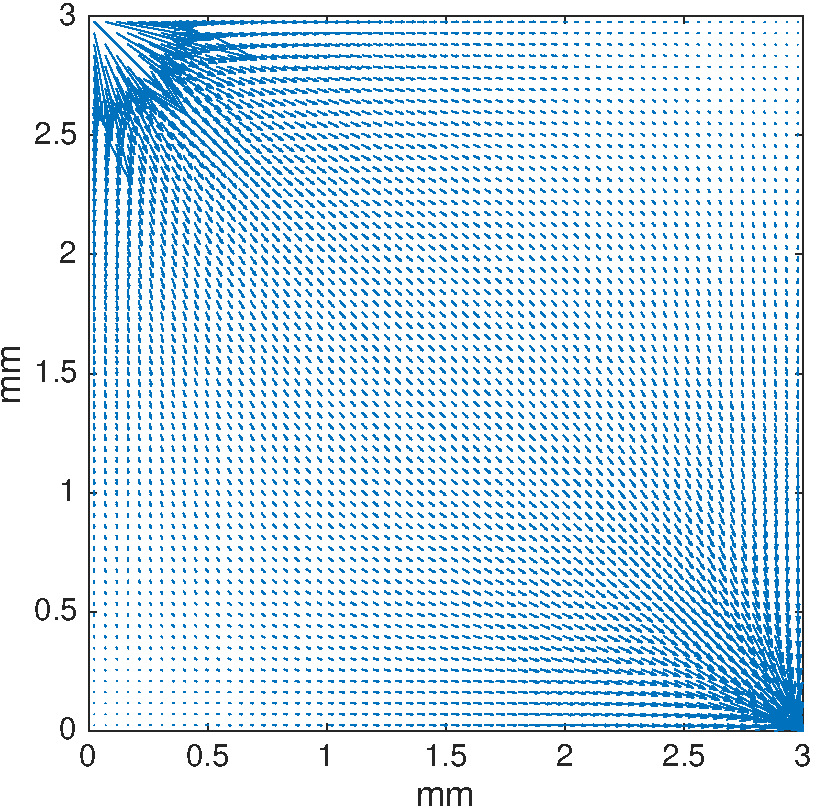
\includegraphics[width=\fwd]{figs/qmat.pdf} & 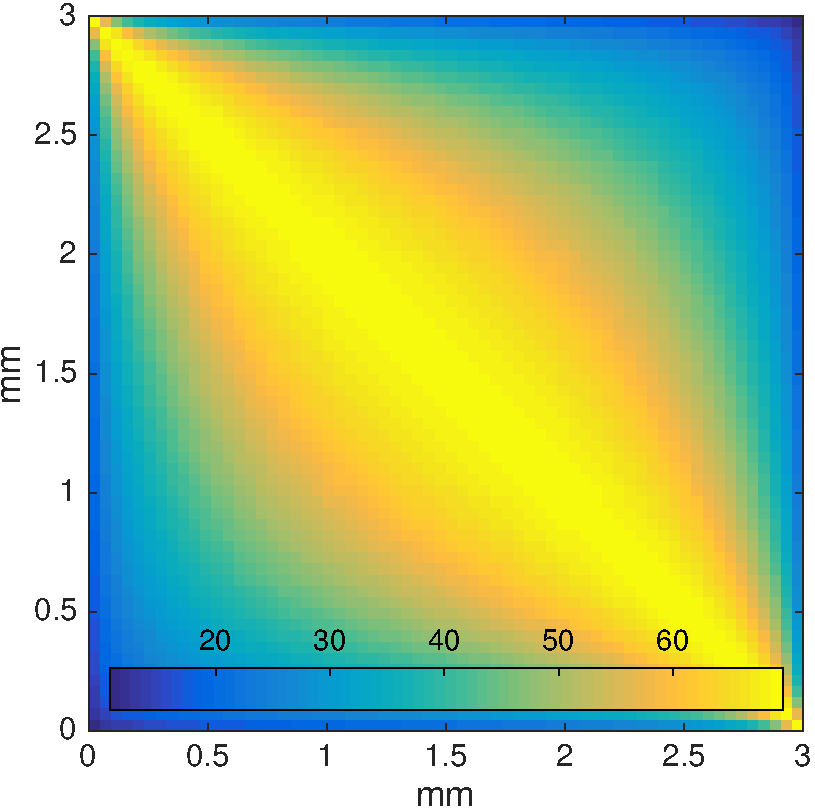
\includegraphics[width=\fwd]{figs/perfmat.pdf} & 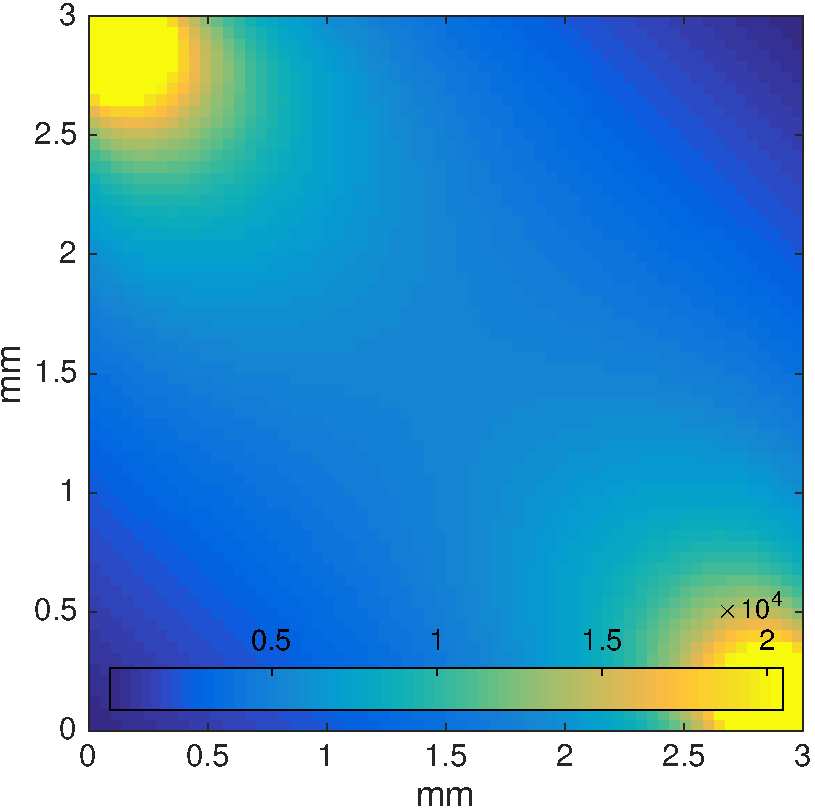
\includegraphics[width=\fwd]{figs/lperfmat.pdf}\\
		(a) Synthetic flow field $\vq(\vx)$ & (b) Perfusion $\Perfs$ along the streamlines  & (c) Local perfusion $\Perfv$.
	\end{tabular}
	\caption{Porous media (PM) flow model with a source in the upper left corner and a sink in the lower right corner. (a) Flow field by the PDE model used to simulate distribution of the contrast agent. (b) Perfusion along the streamlines according to \eqref{eq:flux2perf}. (c) Local perfusion according to \eqref{eq:perflocal}.}
        \label{fig:flowpressureperfusion}
\end{figure*}


%	%--------------------------------------------------
%	%--------------------------------------------------
%	% Section: Results
%	%--------------------------------------------------
%	%--------------------------------------------------
	%\subsection{Results}	
	\subsection{Reconstruction of perfusion within synthetic data}\label{sec:RecPhantom}


	We tested the convolution based traditional model (bSVD) \eqref{eq:conv} as well as maximum-slope (MS) model \eqref{eq:MS} for their capability to recover perfusion, and both models were compared to ground truth perfusion values.
	Prior to reconstruction, the CA concentration map $C(\mathbf{x}_i,t_j)$ was downsampled to a time-resolution of $\SI{.1}{\second}$.
	In order to simulate different spatial resolutions of the scanning process, the data was averaged using different block-sizes ranging from $(1,1)$ pixel (i.e. same resolution as the PDE model) to $(64,64)$ pixels (i.e. entire domain).		
	Success of restoration was measured in terms of averaged relative error of the recovered perfusion with respect to the ground truth perfusion, $RE :=  (\Perf_{\mathrm{rec}} - \Perf_{\mathrm{true}})/\Perf_{\mathrm{true}}\cdot 100\%$.
	The recovered perfusion $\Perf_{\mathrm{rec}}$ was compared against the two perfusion maps $\Perf_{\mathrm{true}}=\{\Perfv,\Perfs\}$ depicted in Figure~\ref{fig:flowpressureperfusion}.

	The local perfusion map $\Perfv$ was set up according to \eqref{eq:perflocal}. 
	Since normalization is performed with respect to voxel size, the values are unrealistically high and will vary with the discretization.
	As \eqref{eq:voxelcurve} shows, this can nevertheless be regarded a valid definition of perfusion since it models the feeding of arterial blood to a control region.

	The global perfusion map $\Perfs$ was set up using the definition along the streamlines \eqref{eq:flux2perf}.
	This definition most accurately reflects the physical perfusion at a given location and shows plausible perfusion values, cf. Figure~\ref{fig:flowpressureperfusion}. As an internal control, the average of $\Perfv$ was found to be \SI{49.59}{\siPml}, for all practical means identical to the global input perfusion of $\SI{50}{\siPml}$.
	However, we do not expect the traditional models to be able to recover these values either.
	To quantify the errors occurring by traditional methods, the global arterial input function was used for the deconvolution, as measured in the source.

	Results from deconvolution by traditional methods are displayed in Table~\ref{tab:resultsSim}. 
	For the complete domain (i.e. block size $64 \times 64$), both the MS method as well as the convolution method were able to restore the ground truth perfusion of \SI{50}{\siPml} accurately with errors of $<1\%$ and $<4\%$ respectively.
	However, the errors are increasing as methods are applied to smaller blocks of the system.
	If compared to $\Perfv$, one can see that results are improving with increasing block size. 
	Note that the block size of $(0.5,0.5)\SI{}{\milli\meter}$ is within the range of resolution available on clinical scanners today. %, and is therefore clinically interesting.
	Also a clear advantage of the bSVD method as compared to MS can be observed for larger block sizes.

	Results from reconstructing the porosity $\phi$ (i.e. CBV) according to \eqref{eq:CBV} are also shown in Table~\ref{tab:resultsSim}. The errors are low, independent of block size.

	\begin{table}[h!tb]
		\scriptsize
		\caption{Mean relative error $RE$ and standard deviation (both in \%) of reconstructed perfusion using traditional methods compared to the ground truth values $\Perfv$, CBV, and $\Perfs$ from the digital phantom. The traditional models MS and bSVD are able to restore the perfusion for the entire domain, but fail when dividing the domain into smaller block sizes. On the other hand, the blood volume $\phi$ is recovered accurately, independent of block size. $\Perfs$ is only defined within a coupled system having streamlines and can therefore not be compared with restored perfusion for the entire domain.
		} 
		\centering
		% \begin{tabular}{p{2cm} c c c c c}
		% 				& \multicolumn{2}{c}{$\Perfv$} & CBV & \multicolumn{2}{c}{$\Perfs$}  \\
		% 	block size (mm)	& bSVD				& MS 			&  		& bSVD				& MS 					\\ \toprule
		% 	(0.05,0.05) 		& -93\%$\pm$4\%	& -98\%$\pm$2\%	& <1\%  & 753\% $\pm$ 926\%	& 124\% $\pm$ 79\%		\\
		% 	(0.23,0.23) 		& -67\%$\pm$16\%& -88\%$\pm$6\%	& <1\% 	& 650\% $\pm$ 757\%	& 114\% $\pm$ 66\% 		\\
		% 	(0.5,0.5) 			& -50\%$\pm$23\%& -79\%$\pm$11\%& <1\% 	& 476\% $\pm$ 507\% & 103\% $\pm$ 51\%		\\
		% 	entire domain   	& 4\%			& <1\%  & <1\%	& 		&
		% \end{tabular}		
		\begin{tabular}{p{.3cm} l l l l l}
			& & \multicolumn{4}{c}{block size (\si{\mm})} \\
										& 		& (0.05,0.05) 		& (0.23,0.23) 	& 	(0.47,0.47)			& Entire ROI \\ \toprule
			\multirow{2}{*}{$\Perfv$}	& bSVD 	& -93\%$\pm$4\% 	& -67\%$\pm$16\%	& -50\%$\pm$23\%	& 4\% 	\\ 
									   	& MS 	& -98\%$\pm$2\% 	& -88\%$\pm$6\%		& -79\%$\pm$11\%	& <1\% 	\\ \midrule
									CBV & 		& <1\% 				& <1\% 				& <1\% 				& <1\% 	\\ \midrule
			\multirow{2}{*}{$\Perfs$}	& bSVD	& 753\% $\pm$ 926\%	& 650\% $\pm$ 757\%	& 476\% $\pm$ 507\% & 		\\
										& MS 	& 124\% $\pm$ 79\%  & 114\% $\pm$ 66\%	& 103\% $\pm$ 51\% 	& 		\\
		\end{tabular}

		\label{tab:resultsSim}
	\end{table}

	
	%--------------------------------------------------
	%--------------------------------------------------
	% Subsection: Results on Real Data
	%--------------------------------------------------
	%--------------------------------------------------	
	\subsection{Reconstruction of perfusion within real data}\label{sec:RealData}
 	Experimental results from Section \ref{sec:RecPhantom} indicate that application of the deconvolution model to patches of tissues would lead to over estimation of blood flow as compared to the overall flow within the volume of interest.
	In order to illustrate that this effect also may be observed on a complete dataset, we applied the deconvolution model to a clinically acquired human perfusion CT dataset of a 56 years old male male admitted with suspicion of stroke to the Radboud University Medical Center in Nijmegen, the Netherlands.
	The perfusion scan was obtained using a Toshiba Aquilon ONE scanner, pixel-size $\SI{0.43}{\milli\meter}\times\SI{0.43}{\milli\meter}$, slice thickness $\SI{0.5}{\milli\meter}$, contrast agent \SI{50}{\milli\litre} Xentix 300, total scan-time \SI{114}{\second}, time resolution ranging from \SI{2.1}{\second} in the early- to \SI{30}{\second} in the late phase of CA uptake.
	Motion correction was performed with respect to the first timepoint using Euler transformations \cite{Mendrik11}.
	The arterial input function was manually selected by a medical expert within the middle cerebral artery (MCA).
	Since we expected to see local over estimation effects mainly for small voxel sizes, the data was processed at full resolution ($512\times512\times320$) voxels. 
	However, in order to deal with noise it was necessary to apply a prior gaussian smoothing with standard deviation of $1$ voxel.	
	Relative concentrations were estimated from the CT signal assuming a spatially independent proportionality constant. The brain tissue was segmented automatically and used as ROI for the perfusion analysis.

	CBF was then estimated voxelwise using a Matlab implementation of bSVD with the global threshold of $4\%$, yielding an average scaled CBF of \SI{64.357}{\milli\litre\per\minute\per100\milli\gram}.
	Furthermore, we estimated the perfusion for the whole volume of interest by averaging the concentration values first and then performing the bSVD with the above configuration, yielding a total scaled CBF of \SI{24.791}{\milli\litre\per\minute\per100\milli\gram}.
	Voxelwise results are depicted in Figure~\ref{fig:RealData}.

	\begin{figure*}[h!tb]\label{fig:RealData}
		\fwd = .215\textwidth
		\centering
		\begin{tabular}{ccc}
		 {\small% This file was created by matlab2tikz.
%
%The latest updates can be retrieved from
%  http://www.mathworks.com/matlabcentral/fileexchange/22022-matlab2tikz-matlab2tikz
%where you can also make suggestions and rate matlab2tikz.
%
\definecolor{mycolor1}{rgb}{0.00000,0.44700,0.74100}%
%
\begin{tikzpicture}

\begin{axis}[%
width=0.951\fwd,
height=0.75\fwd,
at={(0\fwd,0\fwd)},
scale only axis,
xmin=0,
xmax=120,
xlabel={time [s]},
ymin=0,
ymax=250,
ylabel={rel. concentration},
axis background/.style={fill=white}
]
\addplot [color=mycolor1,solid,forget plot,thick]
  table[row sep=crcr]{%
0	0\\
5	4.81948215980018\\
10	11.7249407767123\\
15	109.788176034815\\
20	221.037522824365\\
25	141.890221064755\\
30	49.1060473080009\\
35	27.7167012296253\\
40	34.5042336994668\\
45	46.9343027309933\\
50	38.6517774527303\\
55	37.0988211659761\\
60	37.9793720995833\\
65	38.8599230331905\\
70	39.7404739667976\\
75	40.6210249004048\\
80	41.501575834012\\
85	42.3663391649169\\
90	41.668129828291\\
95	40.969920491665\\
100	40.2717111550391\\
105	39.5735018184132\\
110	38.8752924817873\\
};
\end{axis}
\end{tikzpicture}%} & 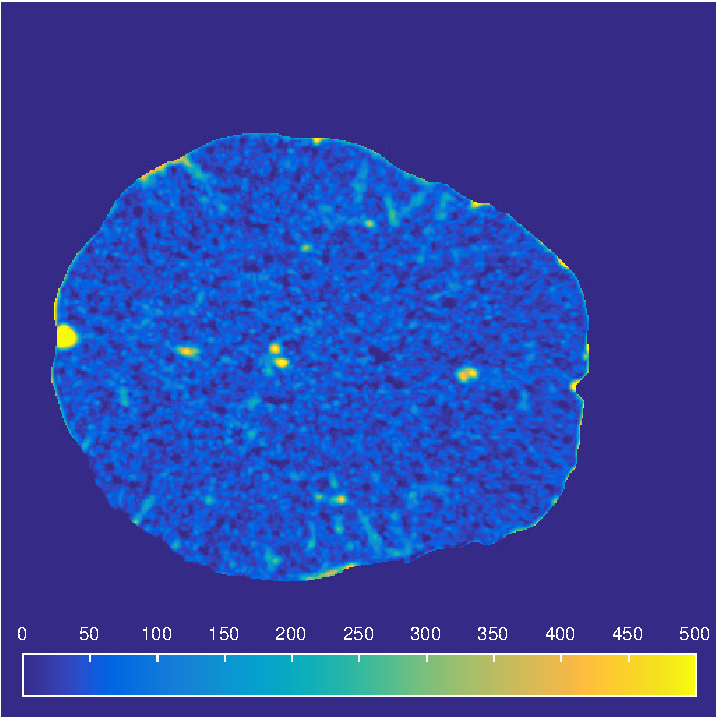
\includegraphics[width = \fwd]{./figs/real_axial160.pdf} & {\small% This file was created by matlab2tikz.
%
%The latest updates can be retrieved from
%  http://www.mathworks.com/matlabcentral/fileexchange/22022-matlab2tikz-matlab2tikz
%where you can also make suggestions and rate matlab2tikz.
%
\begin{tikzpicture}

\begin{axis}[%
width=0.951\fwd,
height=0.75\fwd,
at={(0\fwd,0\fwd)},
scale only axis,
xmin=0,
xmax=250,
xlabel={time [s]},
ymin=-2,
ymax=14,
ylabel={rel. concentration},
axis background/.style={fill=white}
]
\addplot [color=blue,solid,forget plot,thick]
  table[row sep=crcr]{%
0	0\\
5.10888888888889	3.57728482303029\\
10.2177777777778	3.8501111093967\\
15.3266666666667	5.71664126840386\\
20.4355555555556	10.3940019898786\\
25.5444444444444	13.3104878781745\\
30.6533333333333	9.7857007250912\\
35.7622222222222	7.15008816358801\\
40.8711111111111	6.69575791027159\\
45.98	7.0175162477114\\
51.0888888888889	7.11075546536433\\
56.1977777777778	7.06466948033182\\
61.3066666666667	7.08320213588359\\
66.4155555555556	7.1017347914334\\
71.5244444444444	7.12026744698453\\
76.6333333333333	7.13880010253569\\
81.7422222222222	7.15733275808708\\
86.8511111111111	7.17427131128685\\
91.96	7.03339373168847\\
97.0688888888889	6.89251615209099\\
102.177777777778	6.75163857249418\\
107.286666666667	6.61076099289567\\
112.395555555556	6.46988341329856\\
117.504444444444	0\\
122.613333333333	0\\
127.722222222222	0\\
132.831111111111	0\\
137.94	0\\
143.048888888889	0\\
148.157777777778	0\\
153.266666666667	0\\
158.375555555556	0\\
163.484444444444	0\\
168.593333333333	0\\
173.702222222222	0\\
178.811111111111	0\\
183.92	0\\
189.028888888889	0\\
194.137777777778	0\\
199.246666666667	0\\
204.355555555556	0\\
209.464444444444	0\\
214.573333333333	0\\
219.682222222222	0\\
224.791111111111	0\\
229.9	0\\
};
\addplot [color=red,solid,forget plot,thick]
  table[row sep=crcr]{%
0	0.242877310049657\\
5.10888888888889	3.27801404634268\\
10.2177777777778	4.19212893178922\\
15.3266666666667	5.35931224793637\\
20.4355555555556	10.7296350477088\\
25.5444444444444	13.0351453456191\\
30.6533333333333	9.97028747702823\\
35.7622222222222	7.06991667403901\\
40.8711111111111	6.67958740784569\\
45.98	7.10086370332965\\
51.0888888888889	7.00395379245554\\
56.1977777777778	7.14771381111792\\
61.3066666666667	7.0617592832064\\
66.4155555555556	7.04431690009689\\
71.5244444444444	7.24681150319147\\
76.6333333333333	6.97944442254963\\
81.7422222222222	7.29409620580436\\
86.8511111111111	7.12166516958014\\
91.96	6.94933713547804\\
97.0688888888889	7.14300746526767\\
102.177777777778	6.3362801703634\\
107.286666666667	7.15680159666211\\
112.395555555556	5.8535182522262\\
117.504444444444	0.612745947271016\\
122.613333333333	-0.537195282539902\\
127.722222222222	0.406490463075758\\
132.831111111111	-0.24779589623344\\
137.94	0.091958881285865\\
143.048888888889	0.0337330911498852\\
148.157777777778	-0.111471653403876\\
153.266666666667	0.136091537098496\\
158.375555555556	-0.114848569476664\\
163.484444444444	0.0641204450664707\\
168.593333333333	-0.00415036164469126\\
173.702222222222	-0.0465858173026518\\
178.811111111111	0.0758150018721239\\
183.92	-0.0795846098022592\\
189.028888888889	0.061693871067431\\
194.137777777778	-0.0308886810616511\\
199.246666666667	-0.00308806028012709\\
204.355555555556	0.0332184262864778\\
209.464444444444	-0.0574855553444383\\
214.573333333333	0.0790144471363498\\
219.682222222222	-0.104119919783985\\
224.791111111111	0.139008058015951\\
229.9	-0.186333192218881\\
};
\end{axis}
\end{tikzpicture}%} \\
		 (a) & (b) & (c) 
		\end{tabular}
		\caption{Results from real-data experiments (see Sec. \ref{sec:RealData} for details). (a) AIF manually selected from the MCA. (b) One slice of the voxel-wise scaled CBF-reconstruction [\si{\milli\litre\per\minute\per100\milli\gram}] for a 3D volume of interest, cut-off for visualization. (c) Mean concentration curve for the complete 3D volume of interest and the curve approximation by bSVD.}
	\end{figure*}


	
	
	%--------------------------------------------------
	%--------------------------------------------------
	% Section: Discussion
	%--------------------------------------------------
	%--------------------------------------------------	
	\section{Discussion}\label{sec:conclusion}

	
	In this work we have studied the accuracy of traditional 1C models for perfusion reconstruction in a coupled system of blood flow in the capillary system.
	To establish ground truth values, we developed a PDE based digital phantom to simulate blood flow as porous media flow within a slab of capillary tissue.
	%We have justified that the discretized PDE problem can be equivalently described as a system of coupled traditional one-compartment models.	

	Our results strongly support the usage of traditional models for entire regions which are exclusively fed by the measured arterial input.
	However, they also show that if traditional models are applied only to parts of the system, they tend to overestimate the actual perfusion. 
	These limitations are only partly known within the community, and studies reporting voxel wise perfusion maps without discussing their possible limitations are continuously published \cite{Mokin16,Kickingereder15}. 
	Thus, a major motivation for our study is to stimulate the awareness around this topic and to push the development of more appropriate models for future applications.
	%The reason for this is that traditional models do not take into account the correct distribution volume and therefore become discretization dependent.
	

	There are at least two issues related to the overestimation of perfusion. 
	The first issue is that blood passing through a voxel without being locally delivered to the capillary tissue will contribute to artificially high perfusion values. 
	The second issue is thoroughly studied in this work, and relates to estimation of the correct distribution volume used for computing the perfusion. As soon as there is dependency of capillary flow between adjacent voxels, the correct distribution volume used for normalizing the absolute flow into perfusion (i.e. \si{\siPml}) is not known and over-estimation of perfusion will occur. 
	Using local arterial input functions is no remedy for this problem, since the resulting perfusion will depend heavily on the voxel size and overestimate the actual flow, cf. Figure~\ref{fig:perfusion-problem} and \eqref{eq:voxelcurve}.
%	In fact, in the most extreme example we measured overestimated perfusion values which were on average up to $753\%$.
	%JUST ONE NOTE: WE COULD GET ANY VALUE HERE. IF WE GO TO AN EVEN FINER SCALE THE ERROR WIL BE LARGER. WE CAN EVEN PROVE THAT THE ERROR GOES TO INF. WHEN WE APPROACH THE CONTINIOUS SCALE. 

	The results from the digital phantom are supported by real data experiments, where we showed local overestimation of perfusion for small voxel-sizes as compared to an averaging of concentrations for the entire volume of interest.
	Regarding the CBV estimates, one can observe from Table \ref{tab:resultsSim} that estimation of blood volume is far more stable, and  even various block sizes had little impact on the results. 
	These results are in well agreement with the analytical considerations in Section \ref{sec:CBV}, stating that \eqref{eq:CBV} is valid for entire organs as well as for single voxels. 
	Thus, these results support the usage of \eqref{eq:CBV} for computing the CBV with high accuracy for any type of block size, including single voxels.

	Furthermore we have introduced two theoretical definitions of voxelwise perfusion.
	The perfusion $\Perfs$ models perfusion along the streamlines and most accurately reflects the physical notion of volume flow within the correct distribution volume according to mathematical definitions. We showed that $\Perfs$ is a global quantity along the streamline, and scales with streamline length and geometry.
	Theory and experiments show that the traditional models cannot recover this perfusion. The usage of $\Perfs$ for reconstruction of perfusion in real data might as well be challenging as the entire geometry and microscopical flow patterns would have to be known to track the streamlines. However, for our purpose, the concept of $\Perfs$ was useful to clarify the definition of perfusion as a flow that must be normalized along its entire capillary length, where the blood undergoes a transition from arterial to venous blood. 
	For future developments of field models, multi compartment models as suggested in \cite{sourbron14} might be more applicable, where the perfusion was suggested as the non-zero divergence of the arterial flux.

	Perfusion $\Perfv$ was set up based on the interpretation of a coupled system between adjacent voxels. 
	Theory and examples show that this definition of perfusion does not comply with the physical understanding of perfusion since it depends heavily on the discretization.
	However, we have shown that traditional models would restore this local value if the local arterial input function was selected. 
	We have additionally analyzed, both analytically and experimentally, the impact of selecting a further upstream arterial input function.
	Specifically, we have justified that traditional perfusion measurements based on convolution will identify the recursive impulse response function for all upstream voxels (see Section~\ref{sec:NewAndOld}). 
Locally, the correct distribution volume is not accounted for and the obtained perfusion will be overestimated compared to the actual perfusion. The coupling between the continuous model and the convolution model in Section \ref{sec:NewAndOld} demonstrates that the two approaches physically provide the same results, and there is no contradiction between them. The problematic issue of the traditional models is related to physical interpretation and normalization with respect to correct distribution volume.

	
	
	\section{Conclusion}
	In conclusion, our experiments show that traditional methods for perfusion estimation perform well if they are applied to the entire domain.
	For clinical practice this means that perfusion results will be accurate as long as the control volume is independent of all other control volumes.	
%	consists of capillary tissue, where nutrition is delivered, and has direct arterial and venous connection.
	However, if traditional models are applied to only parts of a coupled domain, perfusion becomes scale dependent, resulting in over-estimation of the true value.
	We have illustrated this effect in detail in the case of high resolution images where the voxel size reaches the spatial dimension of the capillary systems, and also showed the effect on real data.
		The reason for this shortcoming is not numerical instabilities in the deconvolution, but rather that perfusion becomes overestimated as traditional models will not account for the correct distribution volume.
  	This problem is expected to become more pronounced in future as imaging hardware is constantly improving in spatial resolution.
	We expect to find overestimation also in pathological tissue, where fluid is passing through multiple, adjacent voxels, and recommend to be take this effect into consideration for clinical evaluation of such data. To account for this problem, the development of new field models for perfusion is therefore highly demanded, in line with approaches described in \cite{sourbron14,Michler2013}. 	

	
	%--------------------------------------------------
	% Bibliography
	%--------------------------------------------------
	\bibliographystyle{IEEEtran}	
	\bibliography{./bibliography}


\end{document}